\documentclass{article}

% Language setting
% Replace `english' with e.g. `spanish' to change the document language
\usepackage[italian]{babel}
\usepackage{verbatim}
\usepackage[utf8]{inputenc}
\usepackage{multicol}
\usepackage{enumitem}


% Set page size and margins
% Replace `letterpaper' with `a4paper' for UK/EU standard size
\usepackage[letterpaper,top=2cm,bottom=2cm,left=3cm,right=3cm,marginparwidth=1.75cm]{geometry}
\usepackage{minted}

% Useful packages
\usepackage{amsmath}
\usepackage{graphicx}
\usepackage[colorlinks=true, allcolors=blue]{hyperref}

\usepackage{listings}
\usepackage{xcolor}
\usepackage{hyperref}

% Impostazioni dello stile del codice
\begin{comment}
\lstdefinestyle{colab}{
    language=Python,
    basicstyle=\ttfamily\small,
    commentstyle=\color[HTML]{398e26},
    keywordstyle=\color{blue},
    numberstyle=\tiny\color{gray},
    numbers=none, % Nessun numero di riga
    frame=none, % Nessun bordo
    backgroundcolor=\color{lightgray!20}, % Sfondo grigio più chiaro
    breaklines=true,
    breakatwhitespace=true,
    showstringspaces=false,
    showtabs=false,
    tabsize=2,
    morecomment=[l]{\#},
}
\end{comment}

\title{AI - Final project}
\author{Piccirilli Michael, Addario Antonio}

\begin{document}
\maketitle

\begin{abstract}
Nel seguente documento vengono riportati i passaggi e gli esperimenti che ci hanno condotto alla costruzione di un modello di regressione in grado di prevedere quando investire e quando vendere utilizzando un algoritmo orientato al Day Trading.

%Si può utilizzare il modello al fine di ottenere una query di valori in cui  scegliere se comprare o investire (guarda immagine di paint), una volta scelto in quali giorni comprare e vendere, partendo dall'ipotesi di avere un'azione di partenza, andiamo a vedere poi con i dati effettivi presenti in y_test, come sarebbe andata se avessimo scelto di vendere quell'azione o di comprarne altre, ossia poi ottenere un valore di portafoglio (se l'azione è stata comprata a 350 e vendota poi quando stava a 300 il portafoglio sarebbe stato di -50)
\end{abstract}

\section{Introduzione}
Al fine di sviluppare un modello che sia adererente ai movimenti della realtà, non ci siamo limitati a sceglierne uno ma abbiamo provato a compararne di diversi scegliendo successivamente quello che minimizzasse determinati errori. Inoltre, dal momento che prevedere l'andamento del prezzo delle azioni risulta essere una pratica complessa e che presenta una moltitudine di variabili da tenere in considerazione, specie per dei neofiti, ci siamo accontentati di un modello che abbia un'accuratezza compresa tra il 50\% e il 60\%. Un'altra considerazione da fare è che il progetto risulta essere un modello giocattolo, perchè non prevede gli andamenti futuri ma ci dà una stima di quello che avrebbe fatto se fosse stato a conoscenza dei valori di apertura, di chiusura ecc. in quel periodo.

\section{Funzionamento}
Il progetto è stato esteso per essere eseguito in 3 modalità differenti:
\begin{itemize}
    \item \textbf{Lato Client: }Il modello viene addestrato (o caricato nel caso in cui sia stato già preaddestrato) sulla propria macchina, è poi possibile vederne i vari grafici e i risultati sulla console dell'ambiente in cui viene eseguito.
    \item \textbf{Lato Server: }Il modello viene caricato ed eseguito su un server virtuale in esecuzione all'interno della macchina. Successivamente, è possibile vederne i risultati attraverso delle \textit{query} effettuabili da un comune browser o attraverso una dashboard costruita ad hoc. 
    \item \textbf{Container:} La terza soluzione offre la stessa modalità di visualizzazione del lato server ma permette l'esecuzione dell'immagine all'interno del container Docker.
\end{itemize}

\section{Esecuzione lato client}
\subsection{Librerie}
Nel seguente frammento di codice vengono mostrate le librerie utilizzate. In particolare:
\begin{itemize}
    \item \textbf{pickle}: libreria che consente di salvare e caricare un modello preaddestrato.
    \item \textbf{pandas, numpy}: librerie che consentono di manipolare i dati (in particolare la prima ci consente di creare strutture dati come DataSet e Series, la seconda ci permette di manipolare array ed effettuare operazioni matematico complesse.
    \item \textbf{yfinance}: libreria che permette di scaricare lo storico della vendita degli stocks. 
    \item \textbf{ta}: librerie per analisi finanziarie.
    \item \textbf{sklearn (scikit-learn)}: libreria che presenta vari modelli di machine learning, permette la scelta delle features migliori, ne calcola l'importanza.
    \item \textbf{xgboost, lightgbm, catboost}: altri modelli di machine learning.
    \item \textbf{optuna}: libreria che permette il tuning degli iperparametri.
    \item \textbf{matplotlib, plotly, seaborn}: librerie per la visualizzazione dei grafici.
\end{itemize}
\begin{minted}[bgcolor=gray!5]{python}
# Per caricare un modello preaddestrato
import pickle

# Gestione dei dati
import pandas as pd
import numpy as np

# Analisi finanziaria
import yfinance as yf
import ta

# Metriche per valutare l'apprendimento
from sklearn.metrics import r2_score, mean_squared_error

# Modelli
from sklearn.linear_model import LinearRegression, Ridge
from xgboost import XGBRegressor
from lightgbm import LGBMRegressor
from catboost import CatBoostRegressor
from sklearn.ensemble import AdaBoostRegressor, ExtraTreesRegressor, 
GradientBoostingRegressor
from sklearn.neighbors import KNeighborsRegressor

# Selezione delle feature
from sklearn.feature_selection import SelectKBest, f_regression

# Tuning degli iperparametri
import optuna

# Gestione dei warning
import warnings

# Visualizzazione dei grafici
import matplotlib.pyplot as plt
import seaborn as sns
import plotly.express as px
import plotly.graph_objs as go
import matplotlib.ticker as mtick

# Libreria per calcolare l'importanza delle features
from sklearn.inspection import permutation_importance
\end{minted}
\newpage
\subsection{Data Preprocessing}
Abbiamo scelto di utilizzare le azioni di Berkshire Hathaway Inc. (BRK-B) che hanno subito una costante crescita di prezzo fino ad oggi.  Utilizziamo quindi la libreria \textbf{yfinance} per scaricare il suo storico e creaiamo un grafico a candela per visualizzare i dati:
\begin{minted}[bgcolor=gray!5]{python}
# Scarica i valori delle azioni di Berkshire Hathaway Inc. 
# (BRK-B) fino alla data odierna
brk = yf.download('BRK-B')

# Crea un grafico a candela delle azioni scaricate
plots.draw_candlestick_plot(brk)
\end{minted}
\begin{figure}[H]
\centering
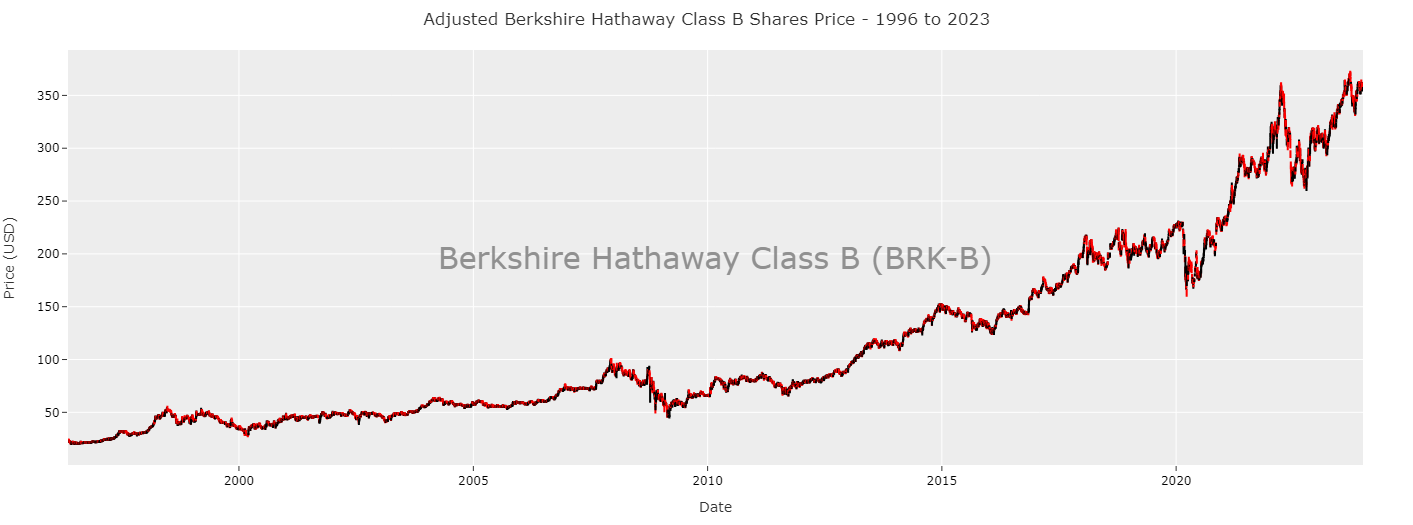
\includegraphics[width=1\linewidth]{candlestick_plot.png}
\caption{\label{fig:candlestick_plot}Grafico a candela delle azioni di Berkshire Hathaway Inc.}
\end{figure}
Si può facilmente vedere che dal 1996 fino ad oggi, il prezzo delle azioni è salito costantemente, confermando ciò che avevamo detto prima, e che ha avuto un picco massimo dal valore di 373.34 \$ per azione il 19 settembre 2023.\\ \\ 
Prima di procedere con le fasi di elaborazione dei dati, dobbiamo dividere il nostro set di dati in set di training e test. Verranno usati i dati dal 1996 al 2016 per addestrare il modello e i dati dal 2017 in poi per testarne le prestazioni.

\begin{minted}[bgcolor=gray!5]{python}
# Divide il DataSet in train e test
train = brk[brk.index.year <= 2016]
test = brk[brk.index.year >= 2017]
\end{minted}
\begin{figure}[H]
\centering
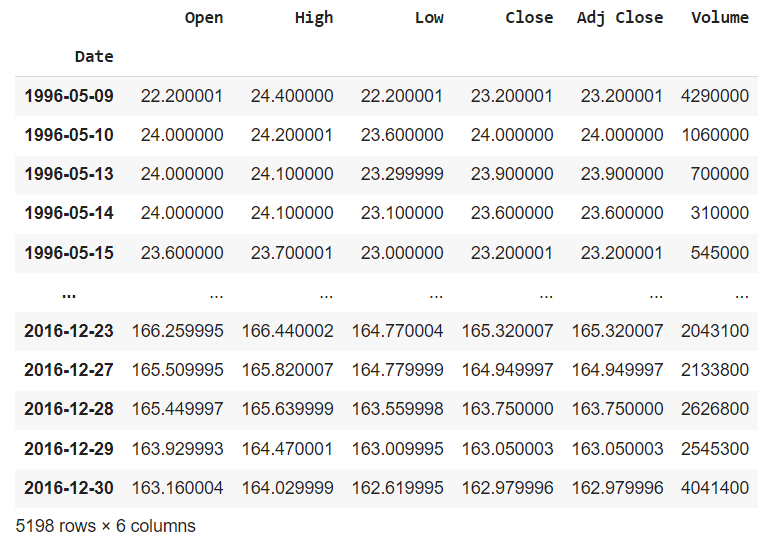
\includegraphics[width=1\linewidth]{train.png}
\caption{\label{fig:train_dataset}DataSet di training con valori dall'inizio della quotazione in borsa al 2017.}
\end{figure}

\subsection{Feature Engineering}
Al fine di rendere il dataset più corposo, abbiamo aggiunto altre features calcolate sulla base di quelle esistenti. In tale modo si riesce ad avere una visione più ampia di quello che è il singolo contesto giornaliero. \\ \\
Infatti, abbiamo creato una funzione chiamata \textbf{feature\_engineering}, che permette quanto detto sopra, per migliorare il potere predittivo dei nostri modelli di regressione. \\ \\
La prima serie di features riflette il comportamento giornaliero dei prezzi: \textbf{High\_low\_ratio} indica la volatilità misurando il rapporto tra il prezzo più alto e quello più basso. \textbf{open\_adjclose\_ratio} cattura la direzione generale del mercato confrontando i prezzi di apertura e di chiusura. Infine, la funzione \textbf{candle\_to\_wick\_ratio} rappresenta la porzione dell'intervallo di prezzo coperto dal “corpo” della candela, ossia la distanza tra i prezzi di apertura e di chiusura di ogni giorno.\\ \\
Le altre caratteristiche sono \textbf{lagged values}, ossia valori ritardati, del prezzo di chiusura rettificato. Spostiamo il prezzo di chiusura di uno, due, tre e cinque giorni indietro per cercare un trend nel passato. Inoltre, calcoliamo il rapporto tra il prezzo di chiusura corrente e i suoi ritardi per catturare il trend e le tendenze in un intervallo di tempo specifico. Ad esempio, un rapporto maggiore di 1 suggerirebbe uno trend rialzista, implicando un potenziale aumento dei prezzi di chiusura nei giorni successivi o addirittura un’inversione dei prezzi. \\ \\
Per analizzare ulteriormente il trend,utilizziamo la libreria \textbf{ta} per calcolare \textbf{medie mobili semplici} per i prezzi di chiusura. Calcoliamo i rapporti tra il prezzo di chiusura e ciascuna media mobile, indicando se il prezzo è superiore o inferiore alla media, fornendo anche informazioni sullo slancio e sulla tendenza attuali. Inoltre, calcoliamo i rapporti tra medie mobili più brevi e più lunghe per catturare lo slancio generale e la tendenza dei prezzi. \\ \\
Aggiungiamo indicatori tecnici classici come \textbf{CCI}, \textbf{RSI} e \textbf{OBV}. 
\begin{itemize}
    \item Il CCI è un indicatore tecnico che può essere utilizzato sia per identificare una nuova tendenza, sia per avvertire condizioni di trading estreme.
    \item L'RSI è un indicatore che segnala la forza intrinseca di un titolo. E' dato dal rapporto tra la media delle sedute borsistiche al rialzo e quelle al ribasso durante un periodo di tempo definito, di solito 14 giorni.
    \item L'indicatore tecnico On Balance Volume (OBV) è un indicatore di analisi tecnica che mette in relazione il volume con le variazioni di prezzo.
\end{itemize}
Creiamo anche altre due funzionalità, catturando le divergenze nell'OBV negli ultimi 10 e 20 giorni. \\ \\
Infine, calcoliamo i rendimenti giornalieri percentuali (\textbf{return\_in\_\%}) e creiamo una variabile target per le previsioni del nostro modello. Si calcola come: 
\begin{equation}
    return\_in\_\% = \frac{Adj\_Close_i - Adj\_Close_{i-1}}{Adj\_Close_{i-1}}
\end{equation}
La variabile \textbf{target} è derivata dai rendimenti giornalieri ma spostata di un giorno indietro. Questo spostamento aiuta il modello a comprendere quali caratteristiche del giorno corrente hanno influenzato i cambiamenti positivi o negativi del giorno successivo.
\begin{center}
    \begin{tabular}{lcr}
    \textbf{date} & \textbf{returns\_in\_\%} & \textbf{target}\\ \\
    1996-05-09 & NaN & 3.45 \\
    1996-05-10 & 3.45 & -0.42 \\
    1996-05-13 & -0.42 & -1.26 \\
    1996-05-14 & -1.26 & -1.69 \\
    1996-05-15 & -1.69 & -2.59 \\
    1996-05-16 & -2.59 & 0.88 \\
    1996-05-17 & 0.88 & -1.32 \\
    1996-05-20 & -1.32 & 0.44 \\
    1996-05-21 & 0.44 & -2.65 \\
    1996-05-22 & -2.65 & 0.45 \\
    \end{tabular}
\end{center}
\begin{comment}
               returns_in_%  target
Date                            
1996-05-09           NaN    3.45
1996-05-10          3.45   -0.42
1996-05-13         -0.42   -1.26
1996-05-14         -1.26   -1.69
1996-05-15         -1.69   -2.59
1996-05-16         -2.59    0.88
1996-05-17          0.88   -1.32
1996-05-20         -1.32    0.44
1996-05-21          0.44   -2.65
1996-05-22         -2.65    0.45
\end{comment}

\begin{minted}[bgcolor=gray!5]{python}
def feature_engineering(df):

    # high_low_ratio indica la volatilità misurata come il rapporto tra i prezzi
    # più alti e più bassi.
    df['high_low_ratio'] = df['High'] / df['Low']

    # open_adjclose cattura la direzione complessiva del mercato confrontando i
    # prezzi di apertura e chiusura.
    df['open_adjclose_ratio'] = df['Open'] / df['Adj Close']

    # candle_to_wick_ratio rappresenta la porzione dell'intervallo di prezzo
    # coperto dal corpo della candela, che rappresenta la distanza tra i 
    # prezzi di apertura e chiusura di ogni giorno.
    df['candle_to_wick_ratio'] = (df['Adj Close'] - df['Open']) / 
    (df['High'] - df['Low'])
    df['candle_to_wick_ratio'] = df['candle_to_wick_ratio']
    .replace([np.inf, -np.inf], 0)

    # I seguenti indici rappresentano il prezzo di chiusura spostato indietro nel
    # tempo di uno, due, tre e cinque giorni.
    df['Close_lag1'] = df['Adj Close'].shift(1)
    df['Close_lag2'] = df['Adj Close'].shift(2)
    df['Close_lag3'] = df['Adj Close'].shift(3)
    df['Close_lag5'] = df['Adj Close'].shift(5)

    # I sequenti valori sono utili per catturare momentum e trend su un determinato
    # arco temporale. Ad esempio, un rapporto superiore a 1 suggerirebbe un 
    # momentum rialzista.
    df['Close_lag1_ratio'] = df['Adj Close'] / df['Close_lag1']
    df['Close_lag2_ratio'] = df['Adj Close'] / df['Close_lag2']
    df['Close_lag3_ratio'] = df['Adj Close'] / df['Close_lag3']
    df['Close_lag5_ratio'] = df['Adj Close'] / df['Close_lag5']

    # Indici che rappresentano la media mobile semplice calcota con finestre di
    # grandezza 10, 20, 80 e 100
    df['sma10'] = ta.trend.sma_indicator(df['Adj Close'], window=10)
    df['sma20'] = ta.trend.sma_indicator(df['Adj Close'], window=20)
    df['sma80'] = ta.trend.sma_indicator(df['Adj Close'], window=80)
    df['sma100'] = ta.trend.sma_indicator(df['Adj Close'], window=100)

    # Rappresentano i rapporti tra il prezzo di chiusura e ciascuna media mobile,
    # indicando se il prezzo è al di sopra o al di sotto della media.
    df['Close_sma10_ratio'] = df['Adj Close'] / df['sma10']
    df['Close_sma20_ratio'] = df['Adj Close'] / df['sma20']
    df['Close_sma80_ratio'] = df['Adj Close'] / df['sma80']
    df['Close_sma100_ratio'] = df['Adj Close'] / df['sma100']

    # Ulteriori indici che rappresentano i rapporti tra le varie medie mobili
    df['sma10_sma20_ratio'] = df['sma10'] / df['sma20']
    df['sma20_sma80_ratio'] = df['sma20'] / df['sma80']
    df['sma80_sma100_ratio'] = df['sma80'] / df['sma100']
    df['sma10_sma80_ratio'] = df['sma10'] / df['sma80']
    df['sma20_sma100_ratio'] = df['sma20'] / df['sma100']

    # Indicatori tecnici del mondo finanziario
    df['rsi'] = ta.momentum.RSIIndicator(df['Adj Close']).rsi()
    df['rsi_overbought'] = (df['rsi'] >= 70).astype(int)
    df['rsi_oversold'] = (df['rsi'] <= 30).astype(int)
    df['cci'] = ta.trend.cci(df['High'], df['Low'], df['Adj Close'], window=20,
    constant=0.015)
    df['obv'] = ta.volume.OnBalanceVolumeIndicator(close=df['Adj Close'], 
    volume=df['Volume']).on_balance_volume()
    df['obv_divergence_10_days'] = df['obv'].diff().rolling(10).sum() - 
    df['Adj Close'].diff().rolling(10).sum()
    df['obv_divergence_20_days'] = df['obv'].diff().rolling(20).sum() - 
    df['Adj Close'].diff().rolling(20).sum()

    # Rapppresenta i rendimenti giornalieri percentuali: calcola la variazione
    # percentuale tra gli elementi successivi della colonna 'Adj Close'. 
    # La formula è (valore_corrente - valore_precedente) / valore_precedente.
    df['returns_in_%'] = np.round((df['Adj Close'].pct_change()) * 100, 2)

    # Variabile target (y) che rappresenta il ritorno in % ma spostato indietro di
    # un giorno al fine di indicare al modello a cosa puntare.
    df['target'] = df['returns_in_%'].shift(-1)

    # Rimuovi i valori null dal DataSet
    df.dropna(inplace=True)

    return df
\end{minted}
Abbiamo applicato la funzione creata sui set di training (\textbf{train}) e testing (\textbf{test}). Dopo aver fatto ciò, abbiamo diviso il dataset in \textbf{features indipendenti(x)} e \textbf{dipendenti(target)}.
\begin{minted}[bgcolor=gray!5]{python}
 # Il DataSet ha bisogno di essere arricchito con ulteriori features in modo
    # da migliorare il potere predittivo del modello
    train = feature_engineering(train)
    test = feature_engineering(test)

    # Divide le variabili indipendenti (X) da quelle dipendendenti (y)
    # axis = 1 indica che stiamo eliminando una colonna (1 per le colonne, 
    # 0 per le righe)
    X_train = train.drop('target', axis=1)
    y_train = train.target
\end{minted}

\subsection{Feature Selection}
I nostri dataset di addestramento e test ora consistono in un totale di 38 attributi dopo aver rimosso la variabile target sia da \textbf{X\_train} che da \textbf{X\_test}.
Sebbene la presenza di numerose features nei nostri dataset con le variabili indipendenti possa aiutare il nostro modello a estrarre il massimo delle informazioni, alcune features potrebbero diventare ridondanti e portare ad un overfitting. Per risolvere questo problema, eseguiremo una \textbf{feature selection univariata} utilizzando \textbf{SelectKBest} di \textbf{Scikit-learn}. Questo metodo seleziona le features in base ai relativi punteggi, in particolare i k punteggi più alti.
\textbf{SelectKBest} applica un test statistico del valore \textit{F} per identificare le features più rilevanti. Nel nostro caso, utilizzeremo come funzione obiettivo \textbf{f\_regression}, che calcola il coefficiente di correlazione di Pearson \textbf{r} tra ciascuna feature e la variabile target continua. È importante notare che \textbf{f\_regression} è adatto solo per variabili target continue e fornisce punteggi F e valori p come risultati.
Per determinare quali caratteristiche selezioneremo, definiremo una soglia per i valori p. Nello specifico, selezioneremo solo quelle caratteristiche il cui valore p è inferiore a 0,2. Questo approccio ci aiuta a concentrarci sulle features che mostrano una relazione statisticamente significativa con la variabile target.
\begin{minted}[bgcolor=gray!5]{python}
    #scegliamo le features migliori
    features = select_features(X_train, y_train, X_test)
\end{minted}
\begin{minted}[bgcolor=gray!5]{python} 
    #funzione per la selezione delle migliori features
    def select_features(X_train, y_train, X_test):
    # Crea un selettore per le feature migliori utilizzando il test F
    k_best = SelectKBest(score_func=f_regression, k=len(X_train.columns))

    # Addestro (e trasformo) il selettettore sui dati di input
    X_train_kbest = k_best.fit_transform(X_train, y_train)
    X_test_kbest = k_best.transform(X_test)

    # Prende gli indici e i nomi delle features
    feature_indices = k_best.get_support(indices=True)
    feature_names = X_train.columns[feature_indices]

    # Salva i valori p, i quali corrispondono ad una feature specifica 
    # e rappresenta la probabilità di osservare
    # la statistica del test F osservata, o una
    #statistica ancora più estrema, supponendo che l'ipotesi nulla sia vera.
    p_values = k_best.pvalues_

    # Creazione features list
    features = []

    # Seleziona solo le features che hanno un valore p minore di 0.2
    for feature, pvalue in zip(feature_names, p_values):
        if pvalue < 0.2:
            features.append(feature)

    # In sintesi, il codice utilizza il test F per valutare la significatività
    # delle feature rispetto alla variabile
    # di output e seleziona solo quelle con valori p
    # al di sotto di una determinata soglia. Questo processo aiuta a
    # identificare le feature più rilevanti per il
    # modello, contribuendo a semplificare e 
    # migliorare la precisione del modello stesso.

    return features
\end{minted}
Le features selezionate risultano essere:
\begin{multicols}{2}
    \begin{itemize}
        \item 'high\_low\_ratio'
        \item 'open\_adjclose\_ratio'
        \item 'Close\_lag1\_ratio'
        \item 'Close\_lag5\_ratio'
        \item 'Close\_sma10\_ratio'
        \item 'Close\_sma20\_ratio'
        \item 'Close\_sma80\_ratio'
    \end{itemize}
    \columnbreak
    \begin{itemize}
    \item 'Close\_sma100\_ratio'
    \item 'sma10\_sma20\_ratio'
    \item 'sma10\_sma80\_ratio'
    \item 'rsi'
    \item 'rsi\_oversold'
    \item 'cci'
    \item 'returns\_in\_\%'
\end{itemize}

\end{multicols}
    
\begin{minted}[bgcolor=gray!5]{python}
    # Crea un nuovo DataSet utilizzando solo le features selezionate
    X_train_kbest = X_train[features]
    X_test_kbest = X_test[features]
\end{minted}

\newpage
\subsection{Modelling}
Abbiamo testato i dati su diversi modelli di regressione per verificare quale fosse il più efficiente a livello di prestazioni. Per questo compito, valuteremo gli algoritmi utilizzando il punteggio $R^2$\textbf{(coefficiente di determinazione)} e l'RMSE \textbf{(Root Mean Squared Error)} .
Il coefficiente di determinazione, indicato come $R^2$, è una misura che fornisce una stima di quanto bene il modello si adatta ai dati di addestramento. Varia tra 0 e 1 dove 1 indica un perfetta adattamento del modello ai dati\footnote{$R^2$ < 0  non è una impossiblità matematica o sintomo di errori, semplicemente significa che il modello scelto si adegua male ai dati}. Il valore $R^2$ rappresenta la frazione della varianza della variabile dipendente che può essere prevista dalle features indipendenti. Un $R^2$ più alto indica una migliore capacità predittiva del modello. La formula di $R^2$ è \[ R^2 = 1 - \frac{\sum_{i=1}^{n}(y_i - \hat{y}_i)^2}{\sum_{i=1}^{n}(y_i - \bar{y})^2} \]
\textit{n}: è il numero totale di osservazioni nel dataset.\\
$y_i$: sono i valori effettivi della variabile dipendente.\\
$\hat{y_i}$: sono i valori previsti dal modello.\\
$\bar{y}$: è la media dei valori effettivi della variabile dipendente.\\

La radice dell'errore quadratico medio (RMSE) è una misura dell'errore medio tra i valori previsti dal modello e i valori effettivi. RMSE penalizza gli errori più grandi in modo più significativo rispetto a quelli più piccoli. La formula di rmse è
\[\text{RMSE} = \sqrt{\frac{1}{n} \sum_{i=1}^{n}(y_i - \hat{y}_i)^2}\]
\textit{n}: è il numero totale di osservazioni nel dataset.\\
$y_i$: sono i valori effettivi della variabile dipendente.\\
$\hat{y_i}$: sono i valori previsti dal modello.\\

Idealmente, stiamo cercando un modello con il punteggio $R^2$ più alto possibile e l'RMSE più basso possibile.
Abbiamo testato i modelli sui dataset con le features selezionate \textbf{X\_train\_kbest} e \textbf{X\_test\_kbest} 
%r2_map, rmse_map = test_models(X_train, y_train, X_test, y_test)
\begin{minted}[bgcolor=gray!5]{python}
r2_mapk, rmse_mapk = test_models(X_train_kbest, y_train, X_test_kbest, y_test)

# Funzione che testa vari modelli di regressione lineare cercandone uno che 
# minimizzi la radice dell'errore quadratico medio e che massimizzi il valore R²
def test_models(X_train, y_train, X_test, y_test):

    # random_state = 42 è un seed che convenzionalmente viene scelto al fine di 
    # riprodurre gli stessi risultati in caso di debug
    regressors = [
        LinearRegression(),
        Ridge(random_state=42),
        ExtraTreesRegressor(random_state=42),
        GradientBoostingRegressor(random_state=42),
        KNeighborsRegressor(),
        XGBRegressor(random_state=42),
        LGBMRegressor(random_state=42, verbose=-1),
        CatBoostRegressor(random_state=42, verbose=False),
        AdaBoostRegressor(random_state=42),
    ]

    r2_map, rmse_map = {}, {}

    # Iterating over algorithms and printing scores
    for reg in regressors:
        reg.fit(X_train, y_train)
        y_pred = reg.predict(X_test)
        r2 = r2_score(y_test, y_pred)
        rmse = mean_squared_error(y_test, y_pred, squared=False)
        ''' print(f'{type(reg).__name__}: R² = {r2:.2f},
        Root Mean Squared Error = {rmse:.2f}')'''
        r2_map[type(reg).__name__] = float(f'{r2:.2f}')
        rmse_map[type(reg).__name__] = float(f'{rmse:.2f}')

    ordered_r2_map = dict(sorted(r2_map.items(), key=lambda item: item[1], 
                                                 reverse=True))
    ordered_rmse_map = dict(sorted(rmse_map.items(), key=lambda item: item[1]))
    return ordered_r2_map, ordered_rmse_map
\end{minted}
\begin{multicols}{2}
\begin{center}
    \textbf{R²}
\end{center}
'LinearRegression': -0.01 \\
'Ridge': -0.01\\
'GradientBoostingRegressor': -0.01\\
'AdaBoostRegressor': -0.04\\
'ExtraTreesRegressor': -0.06\\
'CatBoostRegressor': -0.06\\
'LGBMRegressor': -0.11\\
'XGBRegressor': -0.2\\
'KNeighborsRegressor': -0.22
\columnbreak 
\begin{center}
    \textbf{rmse}
\end{center}
'LinearRegression': 1.33\\
'Ridge': 1.33\\
'GradientBoostingRegressor': 1.34\\
'AdaBoostRegressor': 1.35\\
'ExtraTreesRegressor': 1.37\\
'CatBoostRegressor': 1.37\\
'LGBMRegressor': 1.4\\
'XGBRegressor': 1.45\\
'KNeighborsRegressor': 1.47
\end{multicols}
\begin{center}
    Risultati ottenuti con il dataset contenente solo le feature selezionate
\end{center}
Dal primo test notiamo  come \textit{LinearRegression}, \textit{Ridge} e \textit{GradientBoostingRegressor} totalizzino gli stessi valori di $R^2$ e (approssimativamente) rmse. Per disambiguare tale situazione, abbiamo scelto di operare questi test anche sul dataset completo di tutte le features ottenendo dei risultati molto più promettenti:
\begin{multicols}{2}
\begin{center}
    \textbf{R²}
\end{center}
'GradientBoostingRegressor': 0.01\\
'AdaBoostRegressor': -0.01\\
'CatBoostRegressor': -0.09\\
'ExtraTreesRegressor': -0.11\\
'LGBMRegressor': -0.14\\
'LinearRegression': -0.18\\
'Ridge': -0.24\\
'XGBRegressor': -0.37\\
'KNeighborsRegressor': -0.96
\columnbreak
\begin{center}
    \textbf{rmse}
\end{center}
'GradientBoostingRegressor': 1.32\\
'AdaBoostRegressor': 1.33\\
'CatBoostRegressor': 1.39\\
'ExtraTreesRegressor': 1.4\\
'LGBMRegressor': 1.42\\
'LinearRegression': 1.44\\
'Ridge': 1.48\\'XGBRegressor': 1.55\\
'KNeighborsRegressor': 1.86
\end{multicols}
\begin{center}
    Risultati ottenuti con dataset contenenti tutte le features.
\end{center}
Si nota come il \textit{GradientBoostingRegressor} totalizzi il punteggio migliore sia per l'$R^2$ che per l'rmse. Inoltre, il modello totalizza un punteggio maggiore di $R^2$ e minore di $rmse$ completo di tutte le features rispetto al dataset con features selezionate, denotando come l'ingegnerizzazione delle features non abbia prodotto una maggiore aderenza ai dati reali. Per tale motivo, da qui in avanti, verranno utilizzati i dataset originali per addestrare il modello.\\\\
Vediamo ora come il modello viene allenato con i set di training e come possiamo valutarne l'accuratezza tramite grafici di dispersione.
\begin{minted}[bgcolor=gray!5]{python}
    # Istanzio il modello di regressione
    model_now = GradientBoostingRegressor(random_state=42)

    # Il modello riceve in pasto i dati di allenamento
    model_now.fit(X_train, y_train)

    # Il modello calcola i valori predetti sulla base dei dati di testing
    y_pred = model_now.predict(X_test)

    # Vengono calcolati di nuovo la radice dell'errore quadratico medio e R²
    r2 = r2_score(y_test, y_pred)
    rmse = mean_squared_error(y_test, y_pred, squared=False)

    # Disegna dei grafici di dispersione per vedere come sono distribuiti 
    # le predizioni rispetto ai valori reali
    plots.draw_scatter_plot(y_test, y_pred, r2, rmse)
    plots.draw_frequency_plot(y_test, y_pred)
\end{minted}
\begin{minted}[bgcolor=gray!5]{python}
def draw_scatter_plot(y_test, y_pred, r2, rmse, mode=None):
    plt.scatter(y_test, y_pred)
    plt.xlabel('True Values')
    plt.ylabel('Predicted Values')
    plt.title('True vs. Predicted Values')
    plt.plot([y_test.min(), y_test.max()], [y_test.min(), y_test.max()], 'r--')
    box = dict(boxstyle="round, pad=0.3", fc="white", ec="gray", lw=1)
    plt.text(plt.xlim()[1], plt.ylim()[0] + 0.02, f"R²: {r2:.2f}", ha='right',
    va='bottom', wrap=True, bbox=box)
    plt.text(plt.xlim()[1], plt.ylim()[0] * 0.85 + 0.02, f"RMSE: {rmse:.3f}", 
    ha='right', va='bottom', wrap=True, bbox=box)

    if mode is None:
        plt.show()
    else:
        ...

def draw_frequency_plot(y_test, y_pred, mode=None):
    fig = go.Figure()
    fig.add_trace(go.Scatter(x=np.arange(len(y_test)), y=y_test, mode='lines',
    name='True Values'))
    fig.add_trace(go.Scatter(x=np.arange(len(y_test)), y=y_pred, mode='lines',
    name='Predicted Values'))
    fig.update_layout(title='True vs. Predicted Values', xaxis_title='Index',
    yaxis_title='Values')
    if mode is None:
        fig.show()
    else:
        ...
\end{minted}
\begin{figure}[H]
\centering
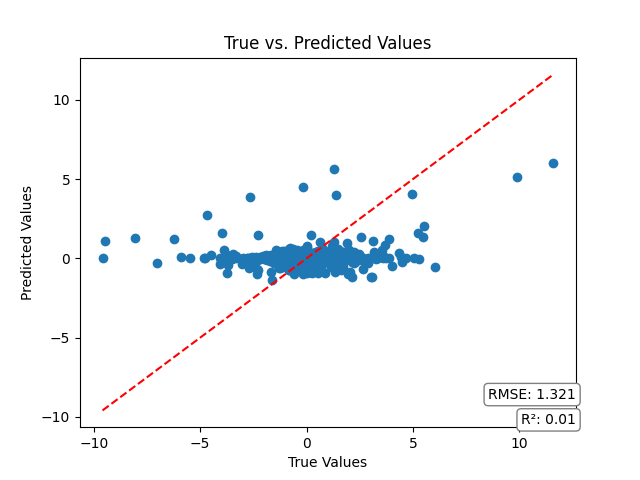
\includegraphics[width=1\linewidth]{Figure_1.png}
\caption{\label{fig:scatter_plot}Grafico di dispersione dei valori reali rispetto a quelli previsti.}
\end{figure}
Sopra è riportato un \textbf{grafico di dispersione} contenente i valori reali in y\_test sull'asse x e i valori previsti in y\_pred sull'asse y.
Nel complesso, la maggior parte dei valori si distribuisce attorno lo 0, un comportamento comune per i dati sui rendimenti giornalieri delle azioni. Tuttavia, è facile notare come il nostro modello abbia difficoltà a prevedere ampi movimenti ribassisti: ci sono punti che dimosrano come le azioni BRK-B siano scese di circa il 10\%, ma il nostro modello prevedeva un rendimento intorno allo 0\%. Lo stesso schema si verifica anche con grandi movimenti rialzisti, i quali però sembrano essere più facili da prevedere, anche se non esattamente nella stessa percentuale del rendimento effettivo. In alcuni giorni in cui le azioni BRK-B sono aumentate del 10\%, il nostro modello prevedeva un aumento di circa il 5\%.
\begin{figure}[H]
\centering
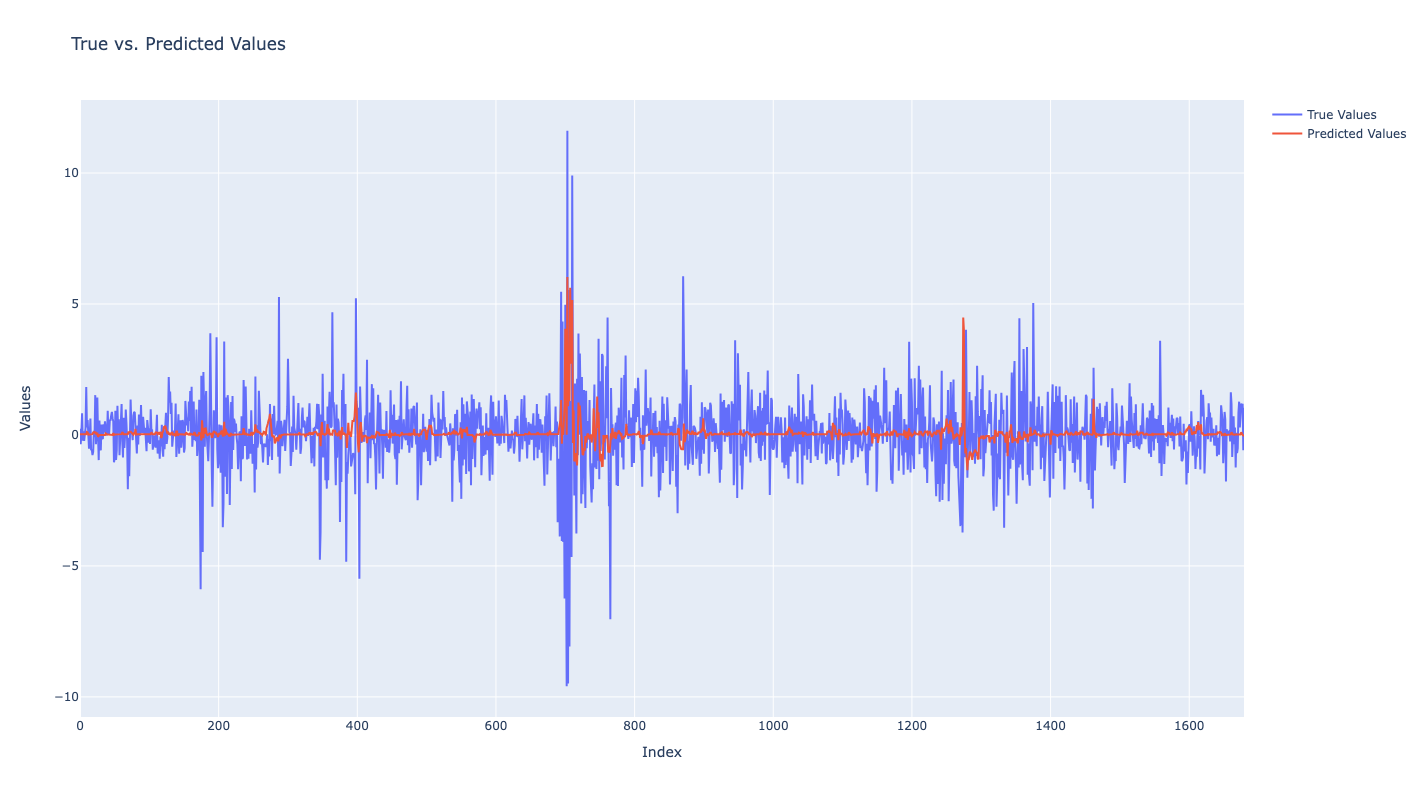
\includegraphics[width=1\linewidth]{newplot.png}
\caption{\label{fig:frequency_plot}Grafico dei rendimenti giornalieri contenente i valori reali e i valori previsti.} 
\end{figure}
I picchi blu rappresentano il movimento reale dell'azione, mentre i picchi rossi quelli predetti dal modello. Anche in questo caso è possibile osservare che il nostro modello fatica a prevedere ampi movimenti verso il basso, ma sembra comunque in grado di prevedere abbastanza bene ampi movimenti verso l’alto. 
\\ \\
Di seguito, possiamo dare un'occhiata al grafico che mostra quanta importanza abbiano le features utilizzate dal modello, ossia le caratteristiche che sono state più utili per prevedere la variabile target.
\begin{minted}[bgcolor=gray!5]{python} 
    # Verifichiamo quanto sono state incisive le feature per i calcoli delle 
    # predizioni
    plots.draw_feature_importance_plot(model_now, X_test, y_test)
\end{minted}
\begin{minted}[bgcolor=gray!5]{python} 
def draw_feature_importance_plot(model, X_test, y_test, mode=None):
    result = permutation_importance(model, X_test, y_test, n_repeats=10,
                                    random_state=42)

    # Calcola la media e ottiene i nomi delle features
    importances = result.importances_mean
    feature_names = X_test.columns

    # Ordina le features in base all'importanza
    indices = importances.argsort()[::1]
    sorted_features = feature_names[indices]
    sorted_importances = importances[indices]

    # Disegna il grafico
    fig, ax = plt.subplots(figsize=(15, 15))
    ax.barh(sorted_features, sorted_importances)
    ax.set_yticklabels(sorted_features)
    ax.set_ylabel('Features')
    ax.set_xlabel('Importance')
    ax.set_title('Feature Importance')
    if mode is None:
        plt.show()
    else:
        ...
\end{minted}
\begin{figure}[H]
\centering
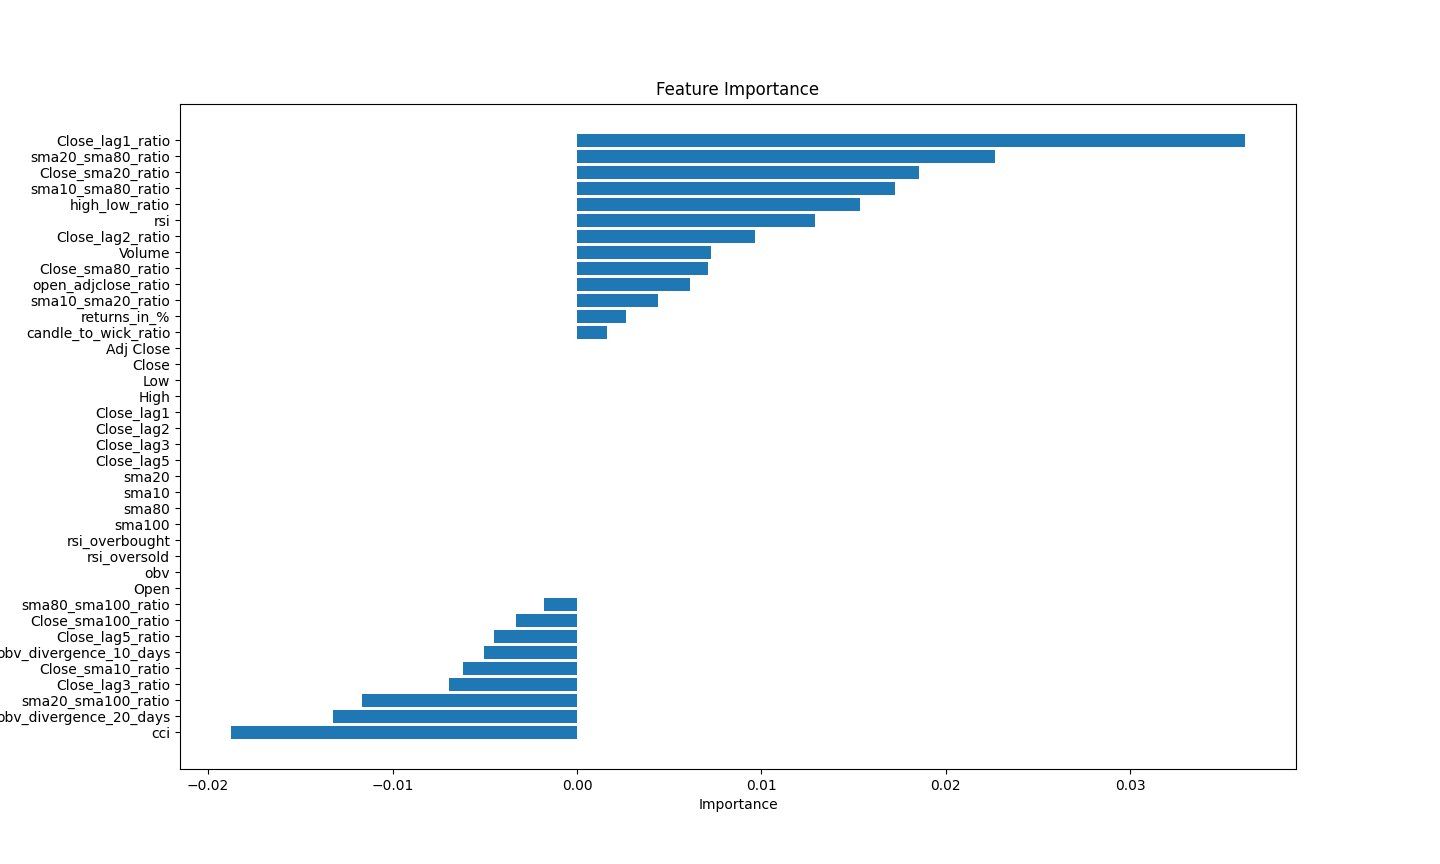
\includegraphics[width=1\linewidth]{FeatureImportance.png}
\end{figure}
La funzione \textbf{permutation\_importance} funziona mescolando casualmente i valori di ciascuna colonna, mantenendo le altre intatte. Questo viene fatto per misurare l'impatto di una modifica di ciascuna colonna specifica sulle previsioni finali. L'importanza sull'asse \textit{x} mostra semplicemente la differenza tra l'accuratezza del set di dati originale e l'accuratezza dopo aver mescolato i valori nelle colonne. Quindi, ad esempio, possiamo vedere che mescolare la colonna \textit{Close\_lag1\_ratio} avrebbe un impatto significativo sulla precisione del nostro modello nell'esecuzione delle previsioni. Infatti, il modello funziona meglio prima di mescolare i dati in questa colonna specifica. Le features con valori di importanza inferiori a 0 semplicemente non influenzano particolarmente le previsioni generali ed indicano che il modello ha prodotto predizioni migliori con quella colonna permutata casualmente piuttosto che con l'ordinamento originale. Ciononostante, non indica necessariamente che le features con valori negativi debbano essere rimosse o alterate. \\ \\
Si può notare, inoltre, che le features create durante l'ingegnerizzazione abbiano un'importanza significativa, specialmente quelle che presentano \textbf{medie mobili}, \textbf{valori ritardati} e \textbf{RSI}. 
\newpage
\subsection{Tuning model}
Per cercare di ottenere punteggi migliori abbiamo pensato di effettuare un'ottimizzazione degli iperparametri mediante l'utilizzo della libreria \textbf{optuna}, che permette di trovare l'impostazione preferibile  dei parametri al fine di ottenere punteggi maggiori. Per iniziare, abbiamo definito la funzione obiettivo, la quale presenta degli argomenti che definiscono il comportamento che il modello dovrà assumere:
\begin{itemize}
    \item \textbf{loss}: testa il modello con diverse funzioni di errore (errore quadratico, errore assoluto, huber e quantile)
    \item \textbf{n\_estimators}: il numero di stimatori, ossia di alberi di decisione che utilizza il GradientBoostingRegressor. Vengono provati un numero di stimatori compreso tra 100 e 1000 con uno step di 50.
    \item \textbf{learning\_rate}: rappresenta il valore di apprendimento del modello, compreso in questo caso tra 0.01 e 0.10.
    \item \textbf{max\_depth}: rappresenta la massima profondita che possono avere gli alberi (compresa tra 3 e 10).
    \item \textbf{min\_sample\_split}: controlla il numero minimo di campioni richiesti per suddividere un nodo interno dell'albero (compreso tra 2 e 20).
    \item \textbf{min\_sample\_leaf}: specifica il numero minimo di campioni richiesti in una foglia (compreso tra 2 e 20).
    \item \textbf{subsample}: indica il numero dei campioni da utilizzare durante l'addestramento di ciascun albero (compreso tra il 10\% e il 100\%)
\end{itemize}
\begin{minted}[bgcolor=gray!5]{python} 
# Funzione obiettivo per il modello
def objective(trial, X_train, y_train, X_test, y_test):
    # Definizione di diversi parametri con cui verrà testato il modello
    params = {
        'loss': trial.suggest_categorical('loss', ['squared_error', 
        'absolute_error', 'huber', 'quantile']),
        'n_estimators': trial.suggest_int('n_estimators', 100, 1000, step=50),
        'learning_rate': trial.suggest_loguniform('learning_rate', 0.01, 0.1),
        'max_depth': trial.suggest_int('max_depth', 3, 10),
        'min_samples_split': trial.suggest_int('min_samples_split', 2, 20),
        'min_samples_leaf': trial.suggest_int('min_samples_leaf', 2, 20),
        'subsample': trial.suggest_uniform('subsample', 0.1, 1.0),
        'random_state': 42
    }

    # Fitting and predicting
    tuning = GradientBoostingRegressor(**params)
    tuning.fit(X_train, y_train)
    preds = tuning.predict(X_test)

    # Computing RMSE score
    rmse = np.round(mean_squared_error(y_test, preds, squared=False), 3)
    return rmse  # Returining the score
\end{minted}
\\
Dopodichè, abbiamo creato un nuovo studio con l'intenzione di ridurre al minimo l'RMSE. La funzione di ottimizzazione prende come input la nostra funzione obiettivo e il numero di tentativi da effettuare (\textbf{n\_trials} = 100): la nostra funzione obiettivo verrà eseguita 100 volte con le impostazioni dei parametri casuali nel dizionario params nella nostra funzione obiettivo riportata di sopra.
\begin{minted}[bgcolor=gray!5]{python} 
    study = optuna.create_study(direction='minimize')
    study.optimize(lambda trial: objective(trial, X_train, y_train, X_test, y_test),
    n_trials=100, show_progress_bar=True)

    # Stampo i valori dei parametri nel miglior trial
    print('Best parameters:', study.best_params)

    # Stampo il minimo valore di RMSE trovato
    print('Best score:', study.best_value)

    # Estrae i risultati dallo studio
    trials = study.trials
\end{minted}
\begin{quote}
\begin{multicols}{3}
    \textbf{Trial 97: Params}\\\\
    {'loss': 'squared\_error'\\
    'n\_estimators': 350\\
    'learning\_rate': 0.0199\\
    'max\_depth': 3\\
    'min\_samples\_split': 17\\
    'min\_samples\_leaf': 3\\
    'subsample': 0.998}\\ \\
    Value - 1.319
\columnbreak \\
\textbf{Trial 98: Params}\\\\
{'loss': 'quantile'\\
'n\_estimators': 450\\
'learning\_rate': 0.0222\\
'max\_depth': 4\\
'min\_samples\_split': 18\\
'min\_samples\_leaf': 2\\
'subsample': 0.895}\\\\
Value - 2.123
\columnbreak \\
\textbf{Trial 99: Params}\\\\
{'loss': 'squared\_error'\\
'n\_estimators': 250\\
'learning\_rate': 0.0155\\
'max\_depth': 3\\
'min\_samples\_split': 20\\
'min\_samples\_leaf': 4\\
'subsample': 0.934}\\\\
Value - 1.315
\end{multicols}
\end{quote}
\begin{center}
    Parametri degli ultimi 3 tentativi per ottimizzare il modello 
\end{center}
Di seguito, viene istanziato nuovamente un GradientBoostingRegressor, passando \textbf{study.best\_params}, in modo che venga eseguito sui migliori parametri per adattarsi ai nostri dati di training e fare previsioni. Quindi, tracciamo ancora una volta un grafico di dispersione confrontando i valori in y\_pred e y\_test.
\begin{minted}[bgcolor=gray!5]{python} 
 # Ristanzio il modello con i parametri ottimizzati
    model_now = GradientBoostingRegressor(**study.best_params)
    model_now.fit(X_train, y_train)

    ...

    model = model_now
    # Da questo momento in poi il codice è condiviso, sia che venga addestrato 
    # che caricato

    y_pred = model.predict(X_test)
    r2 = r2_score(y_test, y_pred)
    rmse = mean_squared_error(y_test, y_pred, squared=False)
    ...

    # A questo punto ridisegnamo i plot di dispersione
    plots.draw_scatter_plot(y_test, y_pred, r2, rmse)
    plots.draw_frequency_plot(y_test, y_pred)

    # Rivisualizziamo come è cambiata l'importanza dele varie feature dopo 
    # l'ottimizzazione
    plots.draw_feature_importance_plot(model, X_test, y_test)
\end{minted}
\begin{figure}[H]
\centering
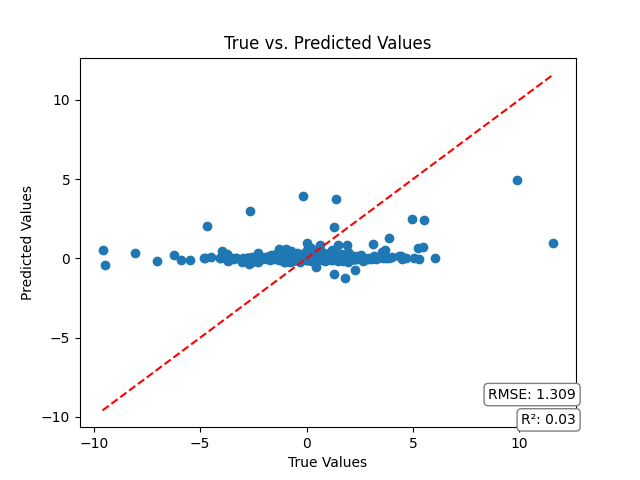
\includegraphics[width=1\linewidth]{scatterPlotOttimizzato.png}
\caption{\label{fig:scatterPlotOttimizzato}Grafico di dispersione calcolato con iperparametri ottimizzati.}
\end{figure}
\begin{figure}[H]
\centering
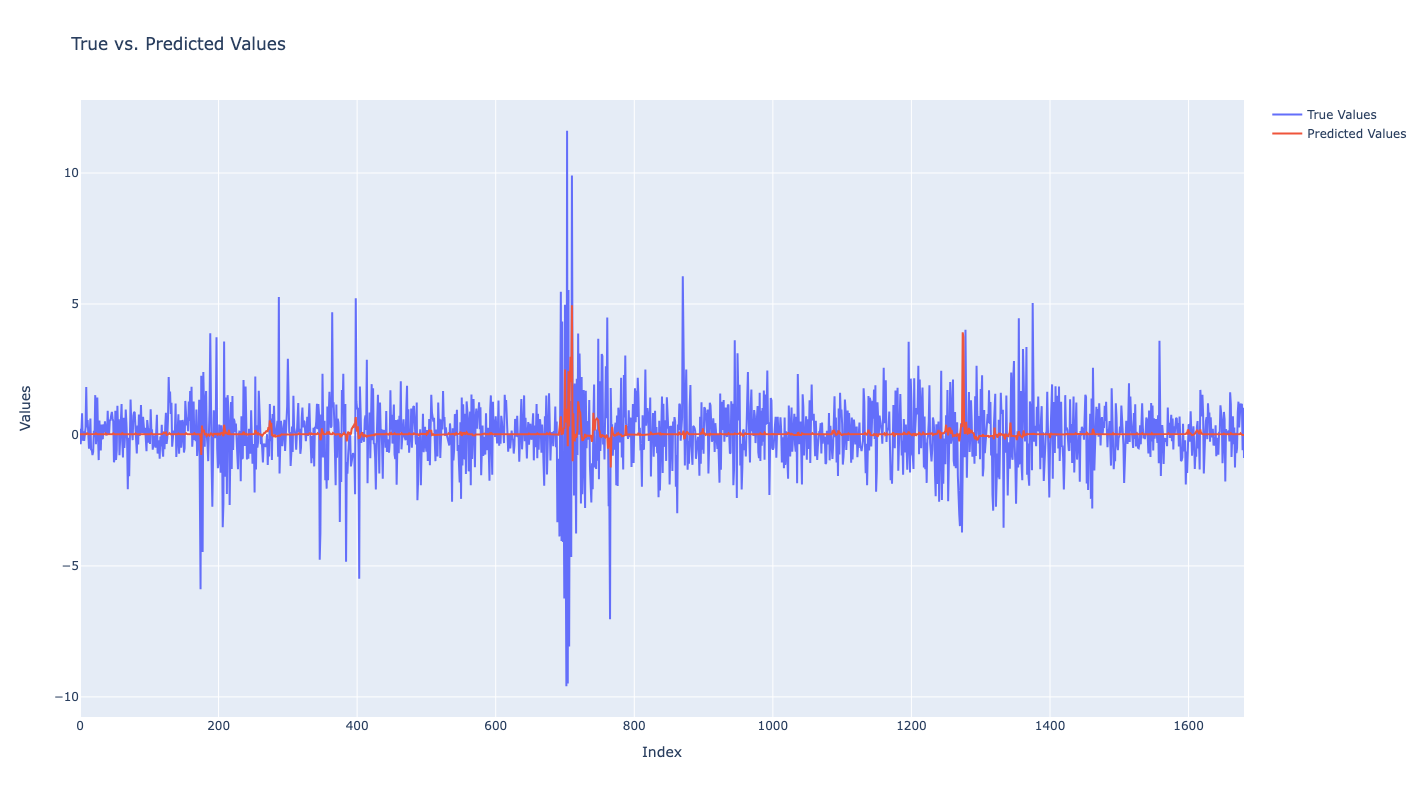
\includegraphics[width=1\linewidth]{frequencyOttimizzato.png}
\caption{\label{fig:scatterPlotOttimizzato}Grafico dei rendimenti giornalieri calcolato con iperparametri ottimizzati.}
\end{figure}
\newpage
Da questi grafici riusciamo subito a notare il miglioramento dopo il tuning degli iperparametri, il valore di \textbf{rmse} è passato da 1.321 a 1.309 e il valore di $R^2$ è aumentato leggermente di 0.02.
Il modello fa ancora fatica a captare ampi rendimenti negativi, ma riesce comunque a prevedere ampi rendimenti positivi.
\begin{figure}[H]
\centering
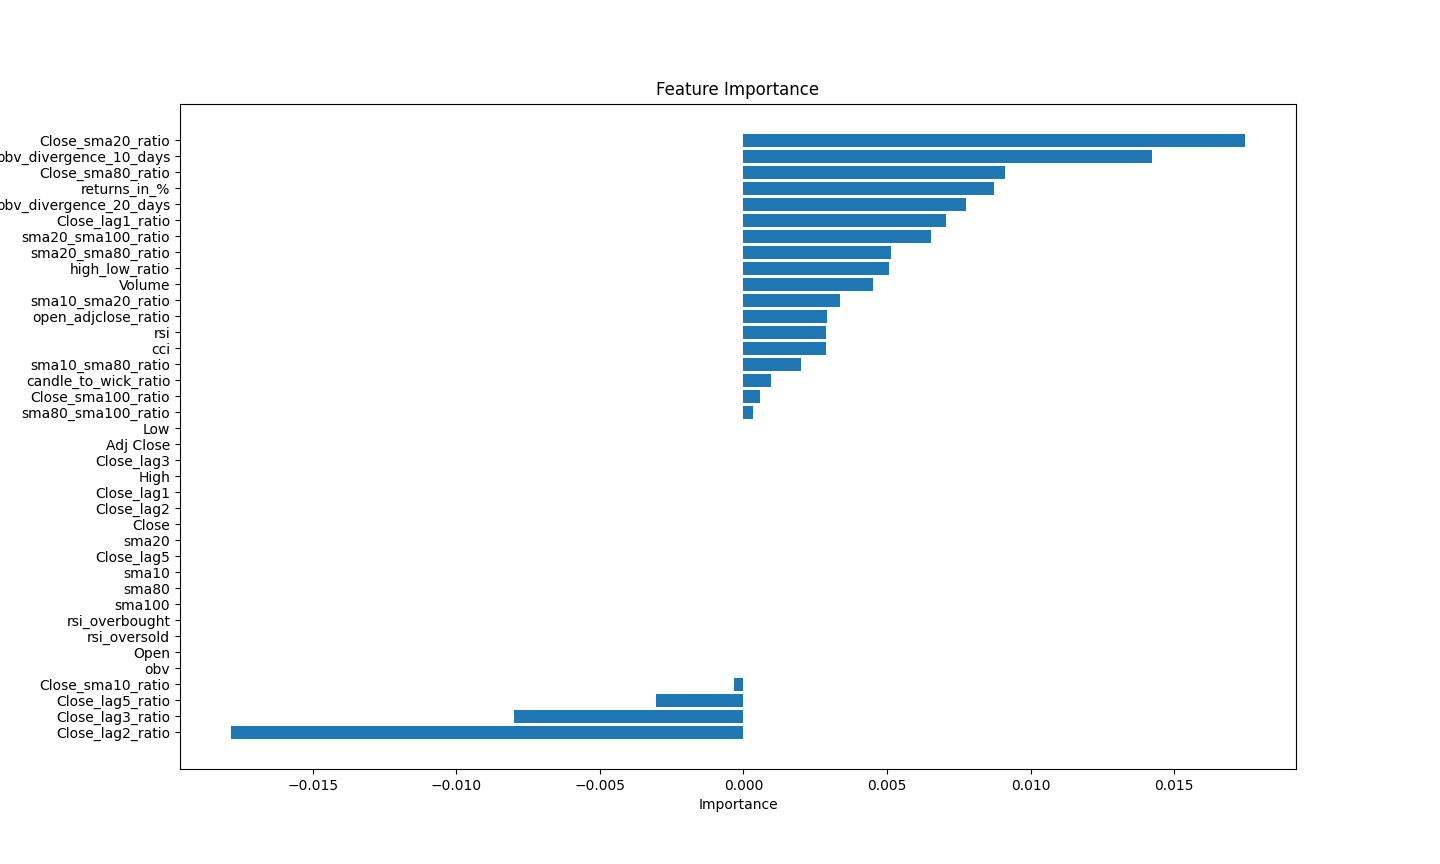
\includegraphics[width=1\linewidth]{featureImportanceOttimizzato.png}
\caption{\label{fig:scatterPlotOttimizzato}Grafico dell'importanza delle features dopo aver migliorato gli iperparametri.}
\end{figure}
Sembra che, questa volta, il \textbf{Close\_sma20\_ratio}, ovvero il rapporto tra il prezzo di chiusura e la media a 20 giorni, sia risultato l'elemento più rilevante. Questa feature è interessante perché può catturare sia la tendenza che il momentum a breve termine. Il momentum viene calcolato misurando la distanza tra il prezzo corrente e la media, mentre il trend identificando se il prezzo corrente è inferiore o superiore alla media. Inoltre, \textbf{Close\_lag1\_ratio} sembra essere altrettanto importante nel modello ottimizzato quanto lo era nel modello originale, così come altre funzionalità create durante il processo di \textbf{feature engineering}.
\newpage
\subsection{Algoritmo di investimento}
\label{subsec:algorithm}
Abbiamo pensato di sviluppare una strategia di investimento orientata al \textbf{Day Trading} acquistando azioni solo nel momento in cui abbiamo una previsione su un possibile trend rialzista (quindi favorevole) e vendendo quando il trend predetto risulta ribassista , mentre negli istanti in cui non ci sono variazioni significative del rendimento, semplicemente non facciamo nulla.
Al fine di comprendere quanto le predizioni siano aderenti alla realtà, abbiamo creato due nuovi dataset utilizzando come threshold lo 0, chiamati \textbf{y\_pred\_class} e \textbf{y\_test\_class} realizzati sulla base degli array \textbf{y\_test} e \textbf{y\_pred}. Tali array presenteranno esclusivamente valori binari, 1 quando il valore è maggiore di 0 e -1 quando è minore.
\begin{minted}[bgcolor=gray!5]{python} 
    y_pred_class = np.where(y_pred > 0, 1, -1)
    y_test_class = np.where(y_test > 0, 1, -1)
\end{minted}
Dopodichè abbiamo costruito una matrice di confusione per analizzare i valori di \textbf{y\_pred\_class} e \textbf{y\_test\_class}. La matrice ci aiuterà a capire con quanta precisione il nostro modello prevede se il giorno successivo le azioni saliranno o scenderanno.
\begin{figure}[H]
    \centering
    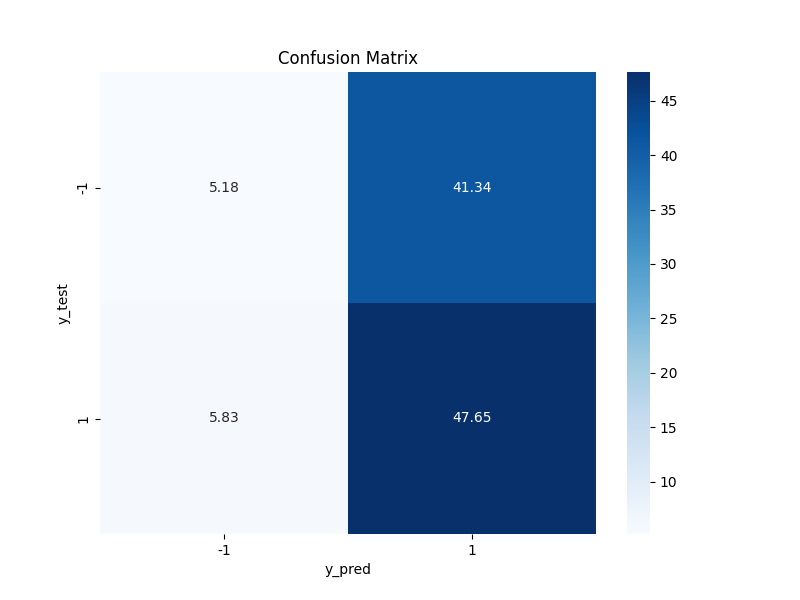
\includegraphics[width=1\linewidth]{confusionMatrix.png}
    \caption{\label{fig:confusionMatrix} Matrice di confusione costruita sui valori 1 e -1 dei dataset.}
\end{figure}
Dalla matrice di confusione emerge che l'\textbf{88.99\%} delle previsioni indica un aumento delle azioni di BRB-K nel giorno successivo. Inoltre, nel \textbf{47.65\%} dei casi in cui il nostro modello prevede un rendimento positivo, il mercato effettivamente registra un aumento di valore per tali titoli.
Globalmente, il nostro modello fornisce previsioni corrette sulla direzione del mercato nel \textbf{53.5\%} dei casi, sia in termini di trend rialzista che ribassista. Tuttavia, è evidente che dimostriamo una maggiore precisione nella previsione di giornate rialziste rispetto a quelle ribassiste.
A questo punto possiamo procedere con la strategia scegliendo un range temporale su cui applicarla.
\begin{minted}[bgcolor=gray!5]{python}
    # Scegliamo un range temporale di cui vogliamo sapere la strategia 
    #(formato 'YYYY-MM-DD')
    time_range = ("2020-12-18", "2021-01-19")

     # Ottengo i risultati dell'algoritmo
    result = make_planning(y_pred, y_test, time_range)

    # Ottengo i prezzi e le azioni messe in atto
    prices, planning = compute_actions(result)

    # Creo il grafico della strategia
    plots.plot_strategy(prices, planning) if display_plot else None
\end{minted}
Definisco il metodo che mi restituirà i risultati dell'applicazione dell'algoritmo: infatti, avrà il compito di preparare il dataframe su cui operare.
\begin{minted}[bgcolor=gray!5]{python}
def make_planning(y_pred, y_test, time_range):
    # Estendo la colonna delle predizioni aggiungendo la data
    # Crea un dataframe combinato con la data e i valori predetti
    y_pred = pd.DataFrame({
        'date': y_test.index,
        'pred': y_pred,
    })
    # Imposto come indice del dataFrame la data
    y_pred = y_pred.set_index("date")
    # print(y_pred)

    result_df = return_strategy(y_pred, time_range)

    return result_df
\end{minted}
Il metodo \textbf{return\_strategy} avrà il compito di operare sul range di tempo scelto e applicare la nostra strategia finanziaria.
\begin{minted}[bgcolor=gray!5]{python}
def return_strategy(_y_pred, time_range):
    start_day, end_day = time_range
    y_pred = _y_pred

    # Applico un treshold alla colonna dei valori predetti
    # Se il valore è positivo allora diventa 1, se è negativo o 0 diventa -1
    y_pred['pred'] = y_pred['pred'].apply(lambda x: 1 if x > 0 else -1)

    # A questo punto ritaglio il dataframe sul range di giorni selezionati
    y_pred = y_pred[start_day:end_day]

    # Creo un array che conterrà i valori della colonna pred
    binary_array = y_pred['pred'].values

    # Creo un valore artificiale per considerare anche l'ultimo elemento,
    # che altrimenti verrebbe tagliato fuori.
    # Tale valore artificiale sarà uguale all'ultimo valore reale
    binary_array = np.append(binary_array, binary_array[len(binary_array) - 1])

    # Creo una lista di coppie (valore, azione)
    result_pairs = []

    # Itero sull'array binario e aggiungo le coppie in base alle inversioni
    for i in range(len(binary_array) - 1):
        current_value = binary_array[i]
        next_value = binary_array[i + 1]

        if current_value == next_value:
            # Se il valore corrente è uguale al successivo, vuol dire che non c'è
            # un'inversione di trend
            result_pairs.append((current_value, "N"))
        elif current_value == 1:
            # Vuol dire che il next_value -1, quindi conviene vendere perchè
            # il giorno successivo il prezzo scenderà
            result_pairs.append((current_value, "V"))
        else:
            # current_value = -1 e next_value 1, quindi compro perchè vuol dire
            # che il giorno successivo il prezzo salirà
            result_pairs.append((current_value, "C"))
    # Creo un nuovo dataframe con i valori e le azioni come colonne
    result_df = pd.DataFrame(result_pairs, columns=['Value', "Action"])

    # Al nuovo dataframe aggiungo la data come indice
    result_df = result_df.set_index(y_pred.index)

    return result_df
\end{minted}
Inizialmente, vengono estratti i giorni di inizio e di termine, viene poi applicata una funzione per rendere la colonna \textit{y\_pred} del dataframe binaria (con valori 1 e -1). Ritaglia quindi il dataframe sul range temporale passato come argomento. Si salva quindi i valori delle predizioni all'interno di un array e aggiunge alla fine dell'array una copia dell'ultimo valore (per considerare anche l'ultimo giorno che altrimenti verrebbe tagliato fuori). Crea quindi una lista vuota in cui aggiunge delle coppie del tipo \textit{(valore, azione)} in base alle inversioni di trend. Possono verificarsi 3 casi:
\begin{itemize}
    \item Il valore corrente è uguale al valore successivo, pertanto viene aggiunta la coppia (current\_value, "N") dove \textbf{N} sta per Niente.
    \item Il valore corrente è 1, ciò significa che il valore successivo è -1, quindi diverso (per forza di cose perchè altrimenti sarebbe entrato nel primo ramo dell'if). Ciò significa che il modello si aspetta che il giorno successivo il prezzo scenda, per tale motivo è meglio vendere prima che questo avvenga. Aggiunge quindi la coppia (current\_value, "V") dove \textbf{V} sta per Vendi.
    \item Il valore corrente è -1 (e quindi il valore successivo è 1 per le motivazioni di sopra). Questo significa che il prezzo per il giorno successivo risalirà, e quindi è meglio acquistare nel giorno corrente. Aggiunge la coppia (current\_value, "C") dove \textbf{C} sta per Compra.
\end{itemize}
\newpage
Il metodo restituisce, quindi, un nuovo dataframe contenente le informazioni essenziali per la strategia: 
\begin{center}
    \textbf{result\_df}\\
    \begin{tabular}{lcr}
    date & Value & Action\\          
    2020-12-18 & 1 & N\\
    2020-12-21 & 1 & N\\
    2020-12-22 & 1 & N\\
    2020-12-23 & 1 & N\\
    2020-12-24 & 1 & N\\
    2020-12-28 & 1 & N\\
    2020-12-29 & 1 & N\\
    2020-12-30 & 1 & N\\
    2020-12-31 & 1 & N\\
    2021-01-04 & 1 & V\\
    2021-01-05 & -1 & C\\
    2021-01-06 & 1 & N\\
    2021-01-07 & 1 & N\\
    2021-01-08 & 1 & N\\
    2021-01-11 & 1 & N\\
    2021-01-12 & 1 & N\\
    2021-01-13 & 1 & N\\
    2021-01-14 & 1 & N\\
    2021-01-15 & 1 & N\\
    2021-01-19 & 1 & N\\
    \end{tabular}
\end{center}
Una volta ottenuto il dataframe, chiamiamo la funzione \textbf{compute\_action()} passando come parametro quest'ultimo. La funzione applicherà le azioni presenti nella colonna \textit{Action} ai prezzi reali dell'azione.
\begin{minted}[bgcolor=gray!5]{python}
  # Ottengo i prezzi e le azioni messe in atto
    prices, planning = compute_actions(result)
\end{minted}
\begin{minted}[bgcolor=gray!5]{python}
def compute_actions(result_df):
    # Estraggo l'intervallo di tempo selezionato
    start_day, end_day = str(result_df.index[0].date()), 
                         str(result_df.index[-1].date())
                         
    # Estendi la data di fine di un giorno (l'ultimo giorno viene escluso)
    extended_end_day = pd.to_datetime(end_day) + pd.DateOffset(days=1)
    brk = yf.download('BRK-B', start=start_day, end=extended_end_day,
                       progress=False)

    # 1. Partiamo con un'azione in possesso
    # e i soldi in negativo per aver comprato l'azione
    # 2. Utilizziamo la variabile money come "portafoglio" per verificare 
    # alla fine quanto abbiamo guadagnato
    # 3. Supponiamo di vendere e comprare sempre al prezzo di chiusura aggiustato
    stocks = 1
    starting_value = brk.loc[start_day, 'Adj Close']
    money = -starting_value
    print(f"\nComprata azione il giorno {start_day} dal valore di 
    {starting_value:.2f}")
    print(f"Portafoglio: {money:.2f}$, Azioni in possesso: {stocks}")

    # Creo un lista di coppie per passare poi i dati alla funzione di plot
    plot_list = [(start_day, starting_value, 'C')]

    # Scorro il DataFrame utilizzando iterrows
    for date, row in result_df.iterrows():
        action = row['Action']
        if action == "V":
            # Se l'azione precedentemente scelta è V di Vendi, 
            # allora cerco il prezzo di chiusura
            # relativo al giorno dell'azione,
            # aggiungo i soldi della vendita al mio portafoglio
            price = brk.loc[str(date.date()), 'Adj Close']
            money += price
            stocks -= 1
            print(f"\nVenduta azione il giorno {str(date.date())} al 
            prezzo di {price:.2f}")
            print(f"Portafoglio: {money:.2f}$, Azioni in possesso: {stocks}")

            plot_list.append((date, price, action))
        if action == "C":
            # Se l'azione precedentemente scelta è C di Compra,
            # allora cerco il prezzo di chiusura
            # relativo al giorno dell'azione
            # e rimuovo dal mio portafoglio i soldi per l'acquisto
            price = brk.loc[str(date.date()), 'Adj Close']
            money -= price
            stocks += 1
            print(f"\nComprata azione il giorno {str(date.date())} al 
            prezzo di {price:.2f}")
            print(f"Portafoglio: {money:.2f}$, Azioni in possesso: {stocks}")

            plot_list.append((date, price, action))

    # Se sono rimaste azioni, converto il valore dell'azione
    # nel rispettivo prezzo di chiusura aggiustato relativo all'ultimo giorno
    while stocks > 0:
        price = brk.loc[end_day, 'Adj Close']
        money += price
        stocks -= 1
        print(f"\nVenduta azione il giorno {end_day} al prezzo di {price:.2f}")
        print(f"Portafoglio: {money:.2f}$, Azioni in possesso: {stocks}")

        plot_list.append((end_day, price, 'V'))

    print("\nResoconto:")
    print(f"Portafoglio: {money:.2f}$, la strategia ha prodotto 
    {'del guadagno' if money > 0 else 'una perdita'}")

    # Converto la lista di prima in un DataFrame
    planning_df = pd.DataFrame(plot_list, columns=['Date', 'Value', 'Action'])
    planning_df['Date'] = pd.to_datetime(planning_df['Date'])
    planning_df.set_index('Date', inplace=True)

    dh.save_data('data_brk', brk[['Adj Close']])
    dh.save_data('planning_df', planning_df)

    return brk[['Adj Close']], planning_df
\end{minted}
Inizialmente manipola i dati passati in modo tale da estrarsi i giorni di inizio e fine dell'intervallo di tempo selezionato (si noti come aggiungiamo anche in questo caso un giorno in più poichè yfinance scarica il dataframe con l'estremo di destra escluso, mentre noi vogliamo includerlo).\\ \\
La funzione utilizza due variabili locali per tenere conto delle informazioni prodotte: \textbf{stocks}, che indica il numero di azioni in possesso e  \textbf{money}, usata come un portafoglio virtuale. \\ \\
A questo punto bisogna stabilire delle regole per l'investimento:
\begin{enumerate}
    \item Partiamo con un'azione in possesso (stocks = 1) e finiamo con 0 azioni.
    \item Partiamo con un credito negativo per aver comprato l'azione (money = -starting\_value).
    \item Compriamo e vendiamo sempre al prezzo di chiusura aggiustato \label{item:terzo}
\end{enumerate}
La (3) è una supposizione molto forte dal momento che, acquistare al prezzo di chiusura aggiustato nello stesso giorno in cui si sta investendo è impossibile. Un'altra opzione valutabile era quella di investire al prezzo di apertura ('Open') o al prezzo dell'azione in quell'istante. \\ \\
Successivamente, inizia il vero e proprio investimento dove vengono lette una ad una le righe del dataframe passato in input (cioè quello prodotto dalla funzione make\_planning()) e vengono valutate le azioni:
\begin{itemize}
    \item Se l'azione è "V", viene salvato il prezzo dell'azione nella variabile price, viene aggiunto tale valore alla variabile money e decrementato il numero di azioni in possesso.
    \item Se l'azione è "C", viene estratto il prezzo dell'azione della data corrente, viene sottratto dalla variabile money e incrementato il contatore delle azioni.
\end{itemize}
Infine, qualora siano rimaste azioni in possesso, queste vengono vendute tutte al prezzo di chiusura aggiustato dell'ultimo giorno dell'intervallo. Il codice è arricchito da funzioni di stampa per tenere traccia degli investimenti che fa la funzione e sono presenti anche varie strutture dati che vengono popolate per permettere poi di creare un grafico riassuntivo.\\\\
\textbf{Output sulla console di compute\_actions:}
\begin{enumerate} 
    \item Comprata azione il giorno 2020-12-18 dal valore di 223.43\\
Portafoglio: -223.43\$, Azioni in possesso: 1

\item Venduta azione il giorno 2021-01-04 al prezzo di 228.45 \\
Portafoglio: 5.02\$, Azioni in possesso: 0

\item Comprata azione il giorno 2021-01-05 al prezzo di 227.47 \\
Portafoglio: -222.45\$, Azioni in possesso: 1

\item Venduta azione il giorno 2021-01-19 al prezzo di 234.55 \\
Portafoglio: 12.10\$, Azioni in possesso: 0
\end{enumerate}
\textbf{Resoconto}: \\
Portafoglio: 12.10\$, la strategia ha prodotto del \textbf{guadagno}.
\newpage
Inoltre, il metodo restituisce due dataframe: \textbf{prices} che presenta la data e i prezzi di chiusura aggiustati e \textbf{planning} che presenta la data, il prezzo relativo all'azione e l'azione eseguita dalla funzione. 
\begin{center}
\begin{multicols}{2}
\begin{center}
    \textbf{prices} \\
\end{center}
\begin{tabular}{cc}
Date & Adj Close \\
2020-12-18 & 223.429993 \\
2020-12-21 & 223.490005 \\
2020-12-22 & 221.880005 \\
2020-12-23 & 224.240005 \\
2020-12-24 & 226.529999 \\
2020-12-28 & 228.410004 \\
2020-12-29 & 229.570007 \\
2020-12-30 & 229.649994 \\
2020-12-31 & 231.869995 \\
2021-01-04 & 228.449997 \\
2021-01-05 & 227.470001 \\
2021-01-06 & 230.270004 \\
2021-01-07 & 232.880005 \\
2021-01-08 & 234.029999 \\
2021-01-11 & 233.429993 \\
2021-01-12 & 233.029999 \\
2021-01-13 & 234.509995 \\
2021-01-14 & 235.020004 \\
2021-01-15 & 233.490005 \\
2021-01-19 & 234.550003 \\
\end{tabular}
\columnbreak
\begin{center}
    \textbf{planning} \\
\end{center}
    \begin{tabular}{lcr}
    Date & Value & Action\\
    2020-12-18 & 223.429993 & C\\
    2021-01-04 & 228.449997 & V\\
    2021-01-05 & 227.470001 & C\\
    2021-01-19 & 234.550003 & V\\     
    \end{tabular}
\end{multicols}
\end{center}
Tali informazioni vengono utilizzate per realizzare un grafico relativo all'andamento della nostra strategia finanziaria.\\
\begin{minted}[bgcolor=gray!5]{python}
    # Creo il grafico della strategia
    plots.plot_strategy(prices, planning) if display_plot else None 
\end{minted}
\label{}
\begin{figure}[H]
    \centering
    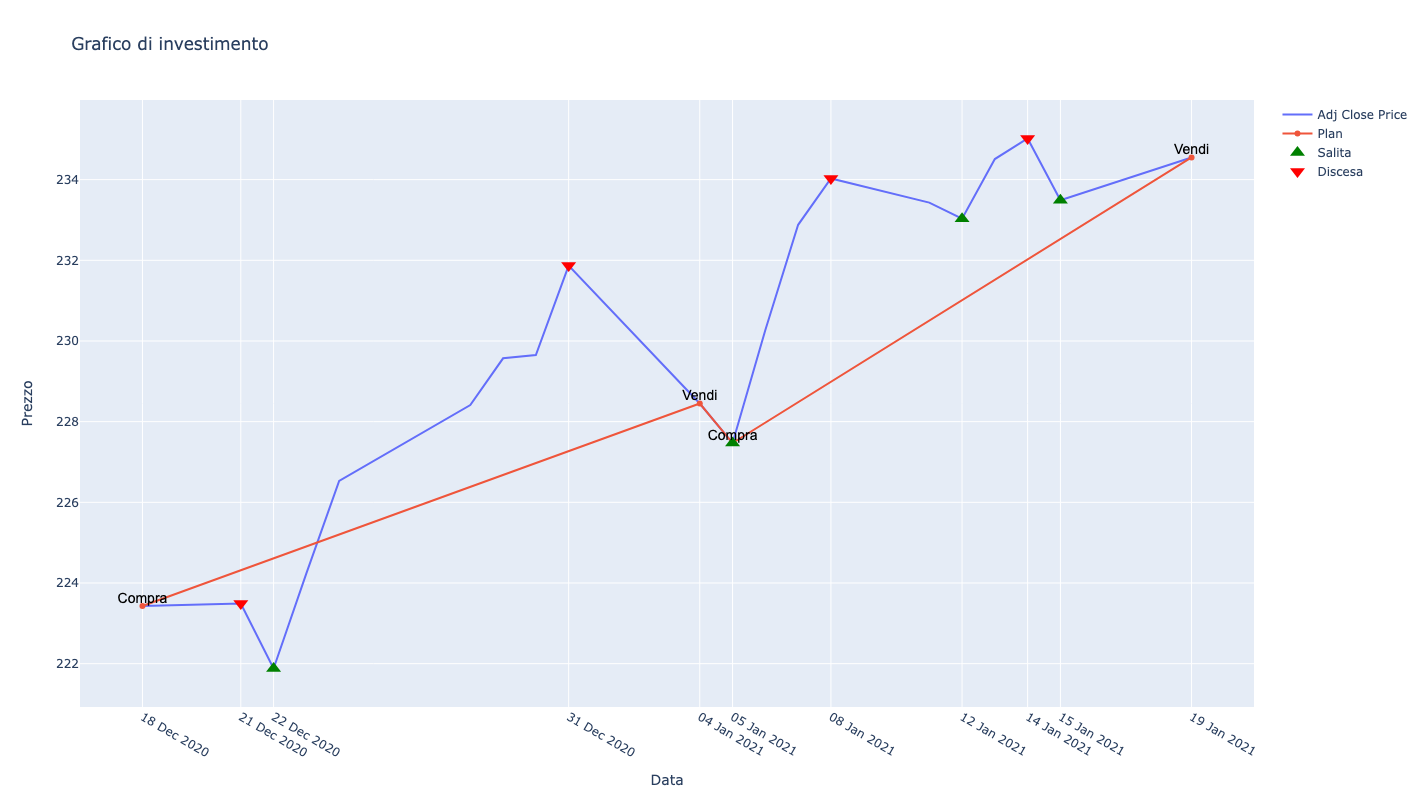
\includegraphics[width=0.90\linewidth]{strategyPlot.png}
    \caption{\label{fig:strategyPlot} Grafico relativo alla strategia finanziaria attuata sull'arco di tempo selezionato.}
\end{figure}
\begin{itemize}
    \item La linea \textcolor{blue}{blu} rappresenta l'andamento dei prezzi di chiusura aggiustati, ad ogni minimo locale è presente un triangolino verde che ci avvisa che il valore dei successivi giorni (finchè non incontrerà un massimo locale) incrementerà. Allo stesso modo, sono presenti triangoli rossi in prossimità dei massimi locali per avvisarci che il trend sarà negativo.
    \item La linea \textcolor{red}{rossa} presenta invece il trend che si è pronosticato il modello. Possiamo notare che, in linea di massima, ha predetto un andamento crescente con una piccola discesa in prossimità di quelli che erano i dati reali, per poi risalire fino alla fine.
\end{itemize}
Ciononostante, esistono intervalli temporali in cui il modello fallisce:
\begin{minted}[bgcolor=gray!5]{python}
    # range di tempo in cui la strategia ci porta ad una perdita
    time_range_fail = ("2020-03-04", "2020-03-20")
\end{minted}
\textbf{Output sulla console di compute\_action:}
\begin{enumerate}
\item Comprata azione il giorno 2020-03-04 dal valore di 217.86 \\
Portafoglio: -217.86\$, Azioni in possesso: 1

\item Venduta azione il giorno 2020-03-12 al prezzo di 175.97 \\
Portafoglio: -41.89\$, Azioni in possesso: 0

\item Comprata azione il giorno 2020-03-13 al prezzo di 196.40 \\
Portafoglio: -238.29\$, Azioni in possesso: 1

\item Venduta azione il giorno 2020-03-20 al prezzo di 170.06 \\
Portafoglio: -68.23\$, Azioni in possesso: 0
     
\end{enumerate}
\textbf{Resoconto}:
Portafoglio: -68.23\$, la strategia ha prodotto una \textbf{perdita}.
\begin{figure}[H]
    \centering
    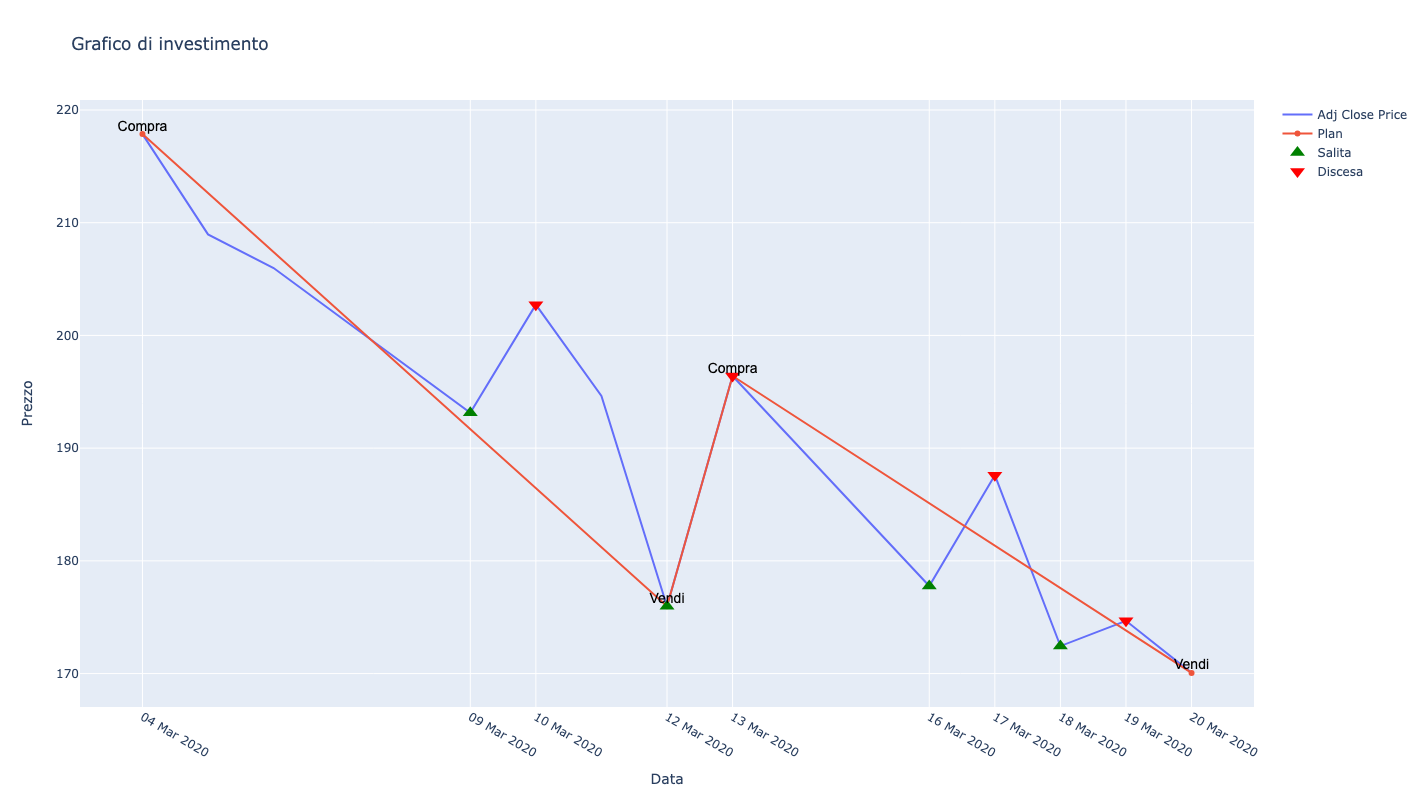
\includegraphics[width=1\linewidth]{strategyPlotFAil.png}
    \caption{\label{fig:strategyPlotFail}Grafico relativo all'andamento della strategia finanziaria nel periodo in cui il modello mostra prestazioni inferiori.}
\end{figure}
In questo grafico, è evidente che il modello commette errori nelle previsioni, portando a perdite significative. Tale scenario era prevedibile anche attraverso l'analisi della matrice di confusione, la quale chiaramente indica la possibilità di predizioni inaccurate, sia nel caso di aumento dei prezzi che diminuzione.
\section{Esecuzione lato server}
Il modello, come precedentemente introdotto, può essere eseguito su un server virtuale lanciabile dal dispositivo stesso che presenta il codice del progetto. Infatti, grazie alla libreria \texttt{Bottle}, è possibile creare un server in ascolto sull'IP \textbf{0.0.0.0:8080} che ci permette di ricevere connessioni in entrata da qualsiasi dispositivo remoto presente nella stessa sottorete\footnote{Per consentire la connessione da qualsiasi dispositivo remoto presente nella sottorete del dispositivo su cui viene eseguito il server, c'è comunque bisogno di aggiungere una regola al Firewall di sistema per permettere connessioni TCP in entrata con porta 8080, inoltre, ciò non potrebbe comunque bastare alla visualizzazione completa della pagina.}. Per facilità di utilizzo, ci connetteremo in locale (usando localhost). Il codice che permette quanto detto sopra è presente nel file \texttt{server.py}. Ora analizziamo cosa permette di fare il server:

\subsection{Avvio del server}
Innanzitutto, viene caricato ed eseguito il modello per poi essere avviato il server grazie al metodo \textbf{run()} della libreria Bottle, passando come parametro l'indirizzo IP da ascoltare, la porta e la modalità (nel nostro caso di debug). Al termine dell'esecuzione, viene riassegnato l'output a quello di sistema con il metoodo cleanup().

\begin{minted}[bgcolor=gray!5]{python}
# Esegui l'app Bottle
try:
    model = load_model()
    run_model(model)
    run(app, host='0.0.0.0', port=8080, debug=True)
finally:
    cleanup()
\end{minted}

A questo punto, possiamo connetterci all'app in localhost attraverso il nostro pc andando in un qualunque browser e digitando l'indirizzo IP \href{http://localhost:8080/}{http://localhost:8080/}

\subsection{Dashboard}
Una volta collegati al server, questo ci ritornerà un file HTML che contiene la dashboard del modello.
\begin{figure}[H]
\centering
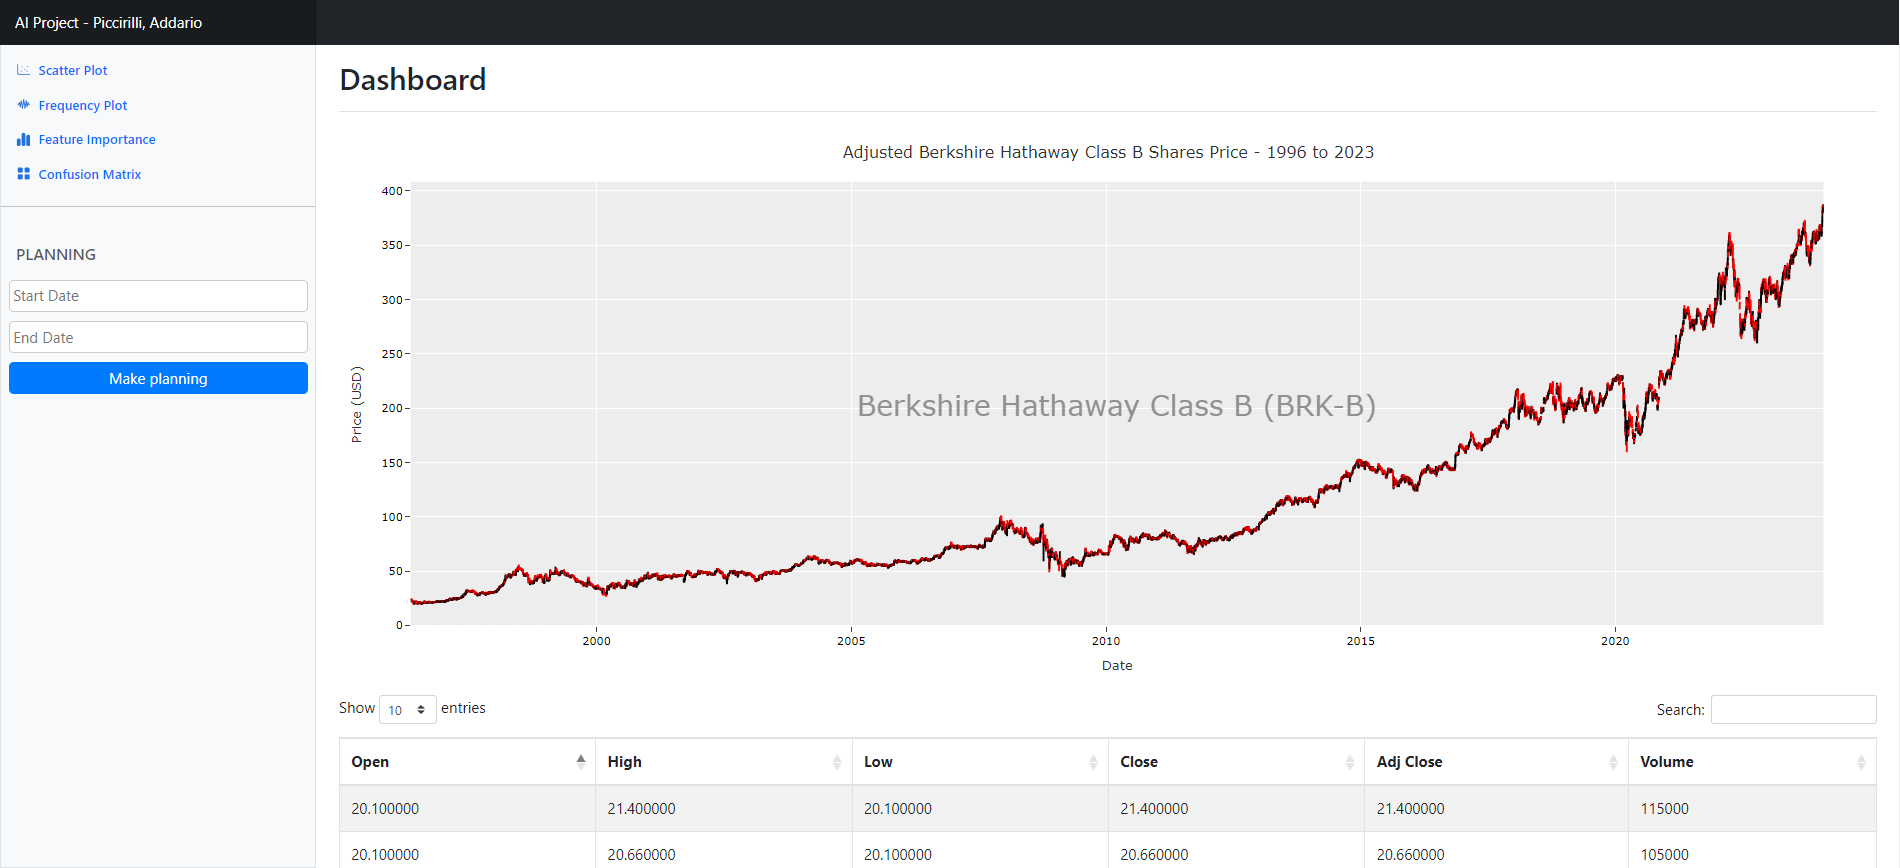
\includegraphics[width=1\linewidth]{dashboard.png}
\caption{\label{fig:train_dataset}Dashboard del progetto.}
\end{figure}
Prima di andare a considerare le varie opzioni che ci permette di vedere la dashboard, analizziamo come il server permette di inviare la pagina web:
\begin{enumerate}
    \item Quando ci colleghiamo all'indirizzo \href{http://localhost:8080/}{http://localhost:8080/}, il server riceve la richiesta GET e cerca il metodo a cui è associata questa richiesta
    \begin{minted}[bgcolor=gray!5]{python}
@app.route('/')
def index():
    # http://localhost:8080/
    with open("web/index.html", "r") as file:
        html_home= file.read()
    return html_home
    \end{minted}
    L'annotazione \textbf{@route} ci permette di mappare uno ad uno i path degli end-point a metodi del server (da qui in avanti, ogni metodo presenterà la sua route per essere eseguito). 
\item All'interno del metodo index() viene letto il file HTML della dashbard e ritornato. Questa presenta due sezioni principali: un menù sulla sinistra con varie opzioni per visualizzare grafici ed effettuare la query di attuazione dell'algoritmo di planning, ed una zona centrale più grande che presenta un grafico a candela dell'andamento dei prezzi di apertura, chiusura, chiusura aggiustata ecc. e, in basso, la tabella con questi valori.
\end{enumerate}
\subsection{Funzionalità}
\subsubsection{Grafici}
Nel menù a sinistra troviamo la possibilità di visualizzare 4 grafici molto importanti per lo studio del modello:
    \begin{enumerate}
        \item \textbf{Scatter plot} o grafico di dispersione 
        \item \textbf{Frequency plot} o grafico di frequenza
        \item \textbf{Feature importance}, ovvere un grafico per visualizzare l'importanza delle varie ferature
        \item \textbf{Confusion Matrix} o matrice di confusione
    \end{enumerate}
Ognuno di questi grafici viene gestito da un metodo che lo crea e lo ritorna come file HTML (nel caso di Plotly) o come immagine (nel caso di Pyplot e Seaborn). Bisogna considerare che per disegnare i vari grafici c'è bisogno delle informazioni legate agli assi, ai punti e ai valori in generale. Per tale motivo si è scelto di utilizzare una sorta di "database" implementato attarverso un dizionario all'interno del file \texttt{data\_handler.py}:
\begin{minted}[bgcolor=gray!5]{python}
shared_values = dict()

def save_data(key, value):
    shared_values[key] = value
\end{minted}
I vari dati vengono salvati man mano che il metodo \textbf{run\_model()} viene eseguito:
\begin{minted}[bgcolor=gray!5]{python}
...
dh.save_data('X_train', X_train)
dh.save_data('y_train', y_train)
dh.save_data('X_test', X_test)
dh.save_data('y_test', y_test)
...
\end{minted}
A questo punto vediamo come viene ritornato un grafico (per comodità scegliamo il metodo che ritorna il frequency plot)
\newpage
\begin{minted}[bgcolor=gray!5]{HTML}
<li class="nav-item">
  <a class="nav-link d-flex align-items-center gap-2" 
  href="/draw_frequency_plot">
  <img src="../web/icons/wave.svg" alt="Wave plot icon" 
  height="16px" width="16px">
    Frequency Plot
  </a>
</li>
\end{minted}
Quando si clicca sulla scritta "Frequency Plot", viene appeso il contenuto del tag \texttt{href} all' url presente nella barra di ricerca per poi essere eseguito. L'url viene mappato grazie all'annotazione @route ed eseguito il metodo ad esso collegato.
\begin{minted}[bgcolor=gray!5]{python}
@app.route('/draw_frequency_plot')
def draw_frequency_plot():
    # http://localhost:8080/draw_frequency_plot
    return plots.draw_frequency_plot(sv['y_test'], sv['y_pred'], 'c')
\end{minted}
Si noti come vengono passati i dati salvati nel data\_handler al metodo per disegnare il grafico insieme ad un carattere \textbf{'c'} che denota la modalità di funzionamento. Questo disegna il grafico e ritorna il file HTML al metodo chiamato dall'url, che a sua volta lo invia al client.
\begin{minted}[bgcolor=gray!5]{python}
def draw_frequency_plot(y_test, y_pred, mode = None):
    ...
    # Disegna il plot
    ...
    if mode is None:
        fig.show()
    else:
        # Ottieni l'HTML del plot
        return fig.to_html(full_html=False)
\end{minted}
Gli altri grafici funzionano allo stesso modo, compreso quello a candela presente nella parte centrale e la tabella subito sottostante.
\subsubsection{Strategia di investimento}
Sempre nel menù a sinistra, è presente una sezione con due campi di testo che ci permettono di inserire delle date. Queste date non rappresentano altro che l'intervallo temporale su cui vogliamo applicare la strategia.
\begin{figure}[H]
\centering
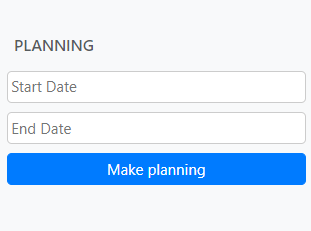
\includegraphics[width=0.30\linewidth]{planning.png}
\caption{\label{fig:planning_menu}Menu di scelta dell'intervallo di tempo.}
\end{figure}
Una volta scelto l'intervallo temporale, basterà cliccare su "Make planning" per ottenere il risultato.
\begin{figure}[H]
\centering
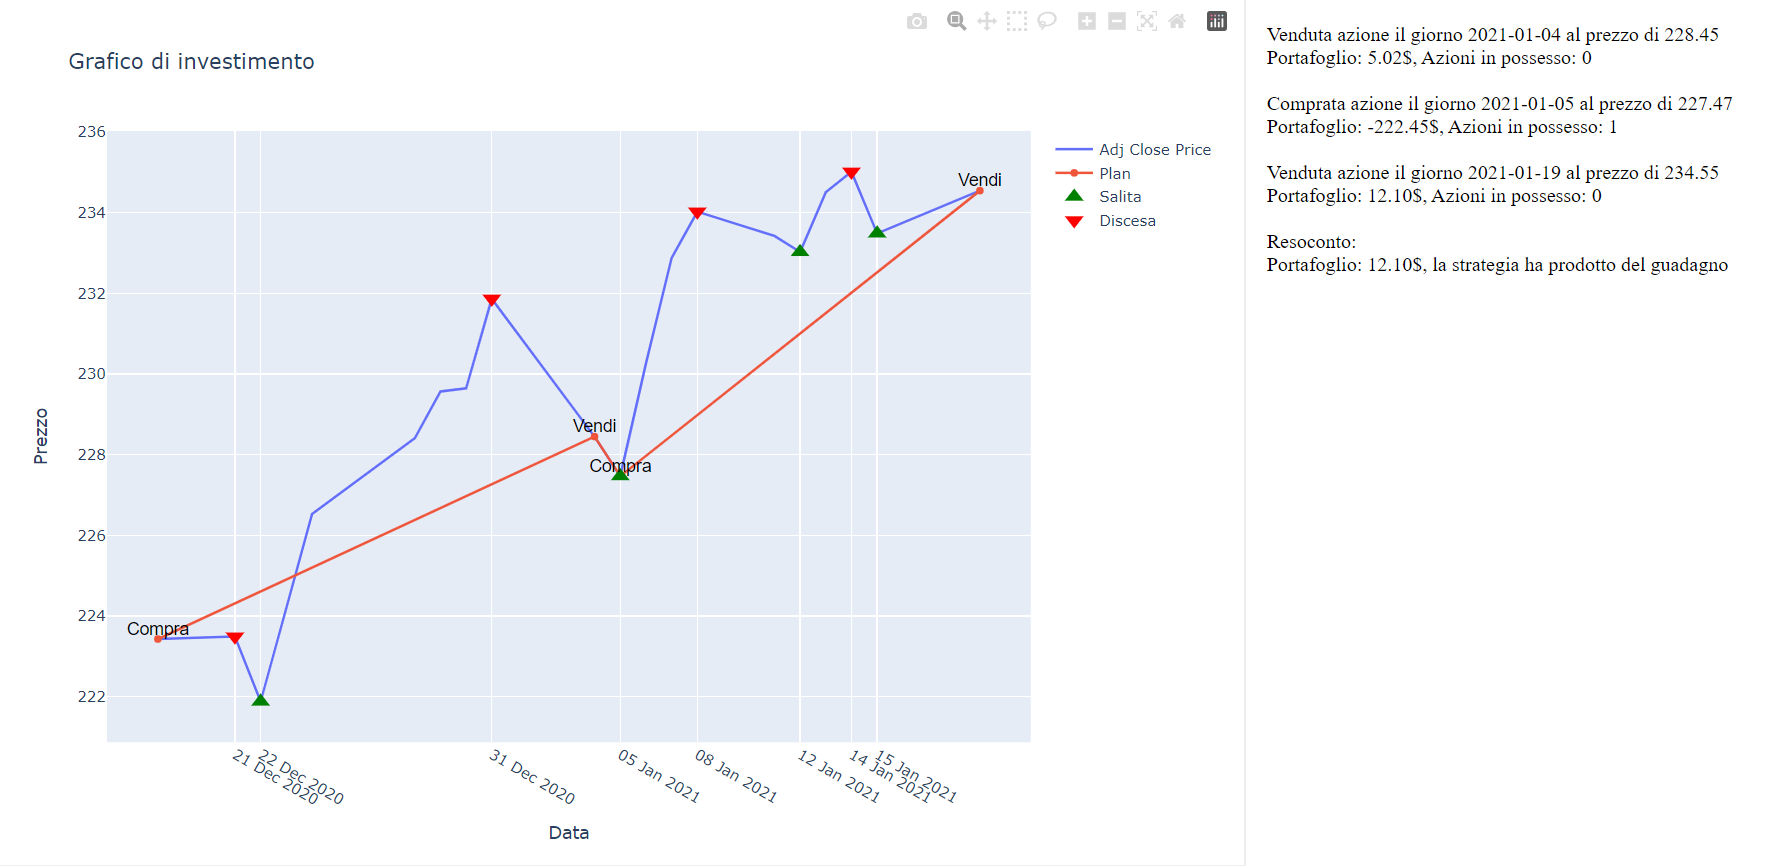
\includegraphics[width=0.85\linewidth]{query_result.png}
\caption{\label{fig:planning_view}Grafico e testo della strategia messo in atto}
\end{figure}
L'analisi del grafico è riportata nella sezione \nameref{subsec:algorithm}
\section{Esecuzione in un container}
Al fine di rendere l'applicativo stand-alone, abbiamo pensato di eseguire il programma all'interno di un container \href{https://www.docker.com/}{Docker}, un servizio che ci permette di costruire un ambiente isolato indipendente dalla macchina su cui è presente. Ciò di cui ha bisogno è unicamente il Docker Engine, presente dopo aver installato Docker Desktop sul proprio dispositivo. Basterà entrare all'interno dell'applicazione di Docker per fare in modo che l'Engine parta in automatico. \\ \\
Al fine di facilitarci la vita abbiamo usato degli script Shell per eseguire i comandi da terminale in modo più rapido:
\begin{minted}[bgcolor=gray!5]{shell}
docker stop ai_project_module
docker rm ai_project_module
docker rmi ai_project_image
docker build -t ai_project_image .
docker run -d --name ai_project_module -p 8080:8080 ai_project_image
docker ps
\end{minted}
Ci soffermeremo poco sulle prime 3 righe dal momento che servono a bloccare ed eliminare eventuali copie del container che stiamo per andare a creare, dedicandoci maggiormente a quelle successive. \\\\
Il comando \textbf{docker build} ci permette di creare un'immagine a partire da un \textbf{Dockerfile}, un file di direttive da dare a Docker (vedremo successivamente il suo contenuto). Specifichiamo con '-t' il nome dell'immagine e selezioniamo con . la cartella di lavoro corrente (quella in cui si trova lo script).\\\\
A questo punto abbiamo costruito l'immagine, ma dobbiamo creare il "contenitore" all'interno del quale essa verrà eseguita. Per tale motivo, utilizziamo il comando \textbf{docker run}, il quale assegna un container all'immagine. L'opzione '-d' permette di specificare che vogliamo eseguire il container in background, l'opzione '- -name' associa un nome al container appena creato, l'opzione '-p' permette di specificare la porta del client (dispositivo su cui viene eseguito il container) e la porta del container. Ciò ci permette di comunicare con il container in entrambe le direzioni. Infine, specifichiamo il nome dell'immagine da assegnare al container.\\ \\
L'ultimo comando, \textbf{docker ps}, stampa semplicemente i container che sono attualmente in esecuzione.\\ \\
Abbiamo affrontato prima come Docker abbia bisogno di istruzioni per generare un'immagine specifica: tali direttive sono presenti all'interno del \textbf{Dockerfile}. Analiziamo riga per riga cosa permette di fare:
\begin{minted}[bgcolor=gray!5, breaklines=true]{docker}
FROM python:3.10-slim
\end{minted}
La prima istruzione è forse la più importante del documento dal momento che ci permette di specificare una base su cui costruire l'immagine: per tale scopo, abbiamo scelto di usare una distribuzione di Python 3.10 presente all'interno di una versione snellita di Debian, sistema operativo basato su UNIX.
\begin{minted}[bgcolor=gray!5, breaklines=true]{docker}
RUN mkdir web
RUN mkdir resources

COPY project.py .
COPY data_handler.py .
COPY server.py .
COPY plots.py .
COPY requirements.txt .
COPY models/model.pkl ./models/
COPY web/ ./web/

# COPY frozen-requirements.txt .
\end{minted}
Le precedenti righe servono per gestire il file system del container: abbiamo bisogno di creare due cartelle, web e resources, con il comando \textbf{mkdir}, e di copiare i file .py che presentano il codice del programma all'interno della root del container (per questo è presente il .). Notiamo come vengano copiati anche un file di "requisiti"\footnote{È presente anche la copia di un file di "requisiti congelati", che contiene il nome delle librerie di cui non abbiamo bisogno avendo il modello preaddestrato. Ciò ci permette di risparmiare un pò di spazio e di velocizzare la fase di installazione delle librerie all'interno del container.}, che presenta le librerie da installare per la corretta esecuzione del modello, e le cartelle che conservano il modello da caricare e i file per la gestione del front-end.
\begin{minted}[bgcolor=gray!5, breaklines=true]{docker}
...
# Aggiorno pip e installo le liberie necessarie
RUN pip install --upgrade pip
RUN pip install --no-cache-dir -r requirements.txt
# RUN pip install -r frozen-requirements.txt
\end{minted}
Come specificato dal commento, i precedenti comandi aggiornano \textbf{pip}, servizio utilizzato per scaricare le librerie di Python presenti all'interno del file \textit{requirements.txt}
\begin{minted}[bgcolor=gray!5, breaklines=true]{docker}
EXPOSE 8080
ENTRYPOINT ["python", "server.py"]
\end{minted}
Queste ultime due righe servono a dire al container di esporre la porta 8080 per comunicare col dispositivo in cui è presente ed eseguire il comando \texttt{python server.py}.\\\\
A questo punto ci bastera eseguire lo script \texttt{mkimage.sh} per lanciare la creazione e l'esecuzione del container.
\begin{table}[h]
\centering
\begin{tabular}{cccccc}
\textbf{CONTAINER ID} & \textbf{IMAGE} & \textbf{COMMAND} & \textbf{CREATED} & \textbf{STATUS} \\ \hline
ca83072d87a4 & ai\_project\_image & "python server.py" & 3 seconds ago & Up Less than a second \\ 
\end{tabular}
\caption{Container Docker attualmente in esecuzione}
\label{tab:my-table}
\end{table}
\end{document}